\documentclass{ieeeojies}
\usepackage{cite}
\usepackage{amsmath,amssymb,amsfonts}
\usepackage{algorithmic}
\usepackage{graphicx}
\usepackage{textcomp}
\usepackage{array}
\usepackage[T1]{fontenc}
\usepackage{xcolor}
\usepackage{multirow}
\usepackage{multicol}
\usepackage{float}
\usepackage{breqn}
\usepackage{url}
\usepackage{times} 
\usepackage{amsmath}
\usepackage{helvet}
\usepackage{ragged2e}
\usepackage{xcolor}
\usepackage{makecell}   


\def\BibTeX{{\rm B\kern-.05em{\sc i\kern-.025em b}\kern-.08em
    T\kern-.1667em\lower.7ex\hbox{E}\kern-.125emX}}

\begin{document}
\title{\centering COMPARATIVE ANALYSIS OF STATISTICAL AND MACHINE LEARNING MODELS FOR ENHANCED CRYPTOCURRENCY PRICE PREDICTION WITH TECHNICAL INDICATOR INTEGRATION}

\author{\uppercase{Le Quoc Khanh}\authorrefmark{1},\uppercase{Le Gia Kiet\authorrefmark{2}, and Nguyen Thi Thuy}\authorrefmark{3}}

\address[1]{Faculty of Information Systems, University of Information Technology, (e-mail: 21520283@gm.uit.edu.vn)}
\address[2]{Faculty of Information Systems, University of Information Technology, (e-mail: 21522255@gm.uit.edu.vn)}
\address[3]{Faculty of Information Systems, University of Information Technology, (e-mail: 25122662@gm.uit.edu.vn)}

\markboth
{Author \headeretal: Le Quoc Khanh, Le Gia Kiet, Nguyen Thi Thuy}
{Author \headeretal: Le Quoc Khanh, Le Gia Kiet, Nguyen Thi Thuy}

\begin{abstract}
    Cryptocurrency price prediction is a challenging yet crucial task in the dynamic realm of financial markets. In this article, we explore the efficacy of various statistical models and machine learning algorithms to forecast cryptocurrency prices. Leveraging a diverse toolkit including Linear Regression, ARIMAX (AutoRegressive Integrated Moving Average with Exogenous Variables), Recurrent Neural Networks (RNN), Gated Recurrent Units (GRU), Long Short-Term Memory (LSTM) networks, Vector Autoregression (VAR), XGBoost, and LightGBM, we aim to capture the complex patterns inherent in cryptocurrency price movements. Technical indicators serve as the primary features, offering insights into market sentiment and trends. Through rigorous evaluation and comparison of these models, we seek to discern their strengths and weaknesses in accurately predicting cryptocurrency prices, contributing to the advancement of predictive analytics in the volatile domain of digital assets.
\end{abstract}

\begin{keywords}
    \textit{Cryptocurrency price, Forecasting, Technical Indicators, Linear regression, ARIMAX, RNN, GRU, LSTM, VAR, XGBoost, LightGBM}
\end{keywords}

\titlepgskip=-15pt

\maketitle

\section{Introduction}
\label{sec:introduction}
\indent Cryptocurrency has become a significant and rapidly growing market, with thousands of different digital currencies available for trading. With the rise of cryptocurrency, there has been an increasing demand for accurate and reliable price prediction models. This paper aims to explore the use of statistical models and machine learning algorithms to predict the price of three popular cryptocurrencies: Bitcoin, Ethereum, and Dogecoin.\\
\indent The price of cryptocurrencies is influenced by a variety of factors, including market demand, investor sentiment, and global economic conditions. These factors make predicting the price of cryptocurrencies a challenging task. However, with the use of statistical models and machine learning algorithms, it is possible to identify patterns and trends in the data that can be used to make more accurate predictions.\\
\indent This paper scrutinizes a comprehensive suite of models, encompassing traditional statistical methods and advanced machine learning algorithms. Specifically, we explore the application of Linear Regression, ARIMAX (AutoRegressive Integrated Moving Average with Exogenous Variables), Recurrent Neural Networks (RNN), Gated Recurrent Units (GRU), Long Short-Term Memory (LSTM) networks, Vector Autoregression (VAR), XGBoost, and LightGBM. We will evaluate the performance of these models using historical price data and assess their ability to accurately predict future price movements.\\
\indent Technical indicators provide valuable insights into market sentiment and trends, aiding in predicting price movements. Integrating these indicators into machine learning models offers a promising strategy to leverage the abundant cryptocurrency market data. This study employs various stock market evaluation indicators, such as moving averages and momentum indicators, to derive features for machine learning. The goal is to enhance predictive accuracy by enabling algorithms to identify meaningful patterns.\\
\indent In summary, by using statistical models and machine learning algorithms to predict the price of cryptocurrencies, investors and traders can make more informed decisions and potentially increase their returns. Additionally, these models and algorithms can be used by cryptocurrency exchanges and financial institutions to manage risk and improve their trading strategies.

\section{Related Works}

\indent There have been multiple studies conducted on the use of statistical models and machine learning algorithms for cryptocurrency price prediction. In a article by Gouxuan Son (2024)\cite{b1}, two models that we concerned in three distinct models employed, Xboost and LightGBM, for predicting Bitcoin prices was conducted. Another paper by Ziyang Yuan (2023)\cite{b2} used KNN, XGBoost and LightGBM to predict the price of Gold and Bitcoin Price. Especially, the investigation found that LightGBM is more effective and space-saving.  Haydier, Albarwari and Ali compared  between  VAR  and  ARIMAX  Time  Series  Models  in Forecasting \cite{b3}. The results showed that the VAR model is better than the ARIMAX model for their observed data depending on the MSE criterion.\\
\indent In another article,\cite{b4} the authors compared the performance of LSTM and GRU models in predicting Bitcoin prices. Additionally, they approved that the GRU model was able to capture long-term dependencies in the Bitcoin price data, while the LSTM model struggled to do so. Meanwhile, \cite{b5} compared and proved that LSTM is also better than RNN.\\
\indent Recent research emphasizes the pivotal role of feature selection in developing effective and interpretable models for cryptocurrency price prediction. Huang, and Ni (2019) \cite{b6} showcased this significance by integrating high-dimensional technical indicators to predict bitcoin returns. Similarly, Mudassir et al. (2020) \cite{b7} employed a machine learning approach using such features for time-series forecasting of Bitcoin prices. These studies underscore the increasing acknowledgment of technical indicators as valuable features in enhancing predictive accuracy within cryptocurrency markets.\\
\indent Based on insights gleaned from numerous prior literature studies, this research aims to predict cryptocurrency prices utilizing a diverse array of predictive models, including Linear Regression, ARIMAX, RNN, GRU, LSTM, VAR, XGBoost, and LightGBM.

\section{Materials}
\subsection{Dataset}
The data is collected from finance.yahoo.com, downloading the daily data of Bitcoin, Ethereum and Dogecoin from 2018-Mar-01 to 2024-Jun-01, including close price, open price, high price, low price, Adjust close and the  volume of trading coins with Currency in USD. \\
Including attributes
\begin{itemize}
    \raggedright
    \item Date: Represents the date of the trading day.
    \item Open: Refers to the opening price of Bitcoin/Ethereum/Dogecoin on that particular day.
    \item High: Indicates the highest price reached by Bitcoin/Ethereum/Dogecoin during that day.
    \item Low: Represents the lowest price reached by Bitcoin/Ethereum/Dogecoin during that day.
    \item Close: Refers to the closing price of Bitcoin/ETH/Dogecoin on that day.
    \item Adj Close: Represents the adjusted closing price, which accounts for factors like dividends and stock splits.
    \item Volume: Refers to the trading volume of Bitcoin on that day, i.e., the total number of Bitcoin/Ethereum/Dogecoin units traded.
\end{itemize}
As the goal is to forecast the price, only data relating to column “Close"
(USD) will be analyzed

\subsection{Descriptive Statistics}

\begin{table}[H]
    \centering
    \renewcommand{\arraystretch}{1.2} % Increase row spacing by 20%
    \newcolumntype{R}{>{\raggedleft\arraybackslash}r} % Define new right-aligned column
    \begin{tabular}{|c|r|r|r|}
        \hline
                & \multicolumn{1}{c|}{\textbf{BTC}} & \multicolumn{1}{c|}{\textbf{ETH}} & \multicolumn{1}{c|}{\textbf{DOGE}} \\
        \hline
        Count    & 2285.000 & 2285.000 & 2285.000 \\
        \hline
        Mean     & 24483.298 & 1383.339 & 0.071 \\
        \hline
        Median   & 18251.604 & 1197.595 & 0.091 \\
        \hline
        Mode     & 3236.762 & 84.308 & 0.002 \\
        \hline
        Min      & 8601.796 & 233.028 & 0.003 \\
        \hline
        25\%     & 20041.738 & 1274.619 & 0.059 \\
        \hline
        50\%     & 37849.664 & 2088.574 & 0.089 \\
        \hline
        75\%     & 73083.500 & 4812.087 & 0.685 \\
        \hline
        Max      & 20041.738 & 1274.619 & 0.059 \\
        \hline
        Std      & 6741.750 & 3156.510 & 0.003 \\
        \hline
        Variance & 333121045.601 & 1434232.661 & 0.008 \\
        \hline
        Kurtosis & 69846.738 & 4727.779 & 0.683 \\
        \hline
        Skewness & 0.762 & 0.703 & 2.005 \\
        \hline
        Range    & -0.509 & -0.528 & 5.603 \\
        \hline
    \end{tabular}
    \caption{Descriptive Statistics of Cryptocurrencies}
    \label{table:1}
\end{table}

\begin{figure}[H]
    \centering
    \begin{minipage}{0.23\textwidth}
        \centering
        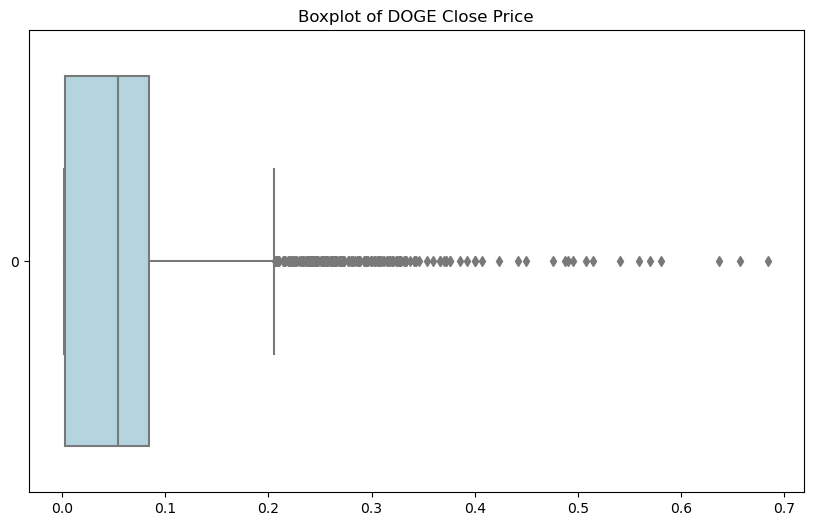
\includegraphics[width=\linewidth]{graph/doge_boxplot.png}
        \caption{DOGE's Box Plot}
        \label{fig:1}
    \end{minipage}
    \hfill
    \begin{minipage}{0.23\textwidth}
        \centering
        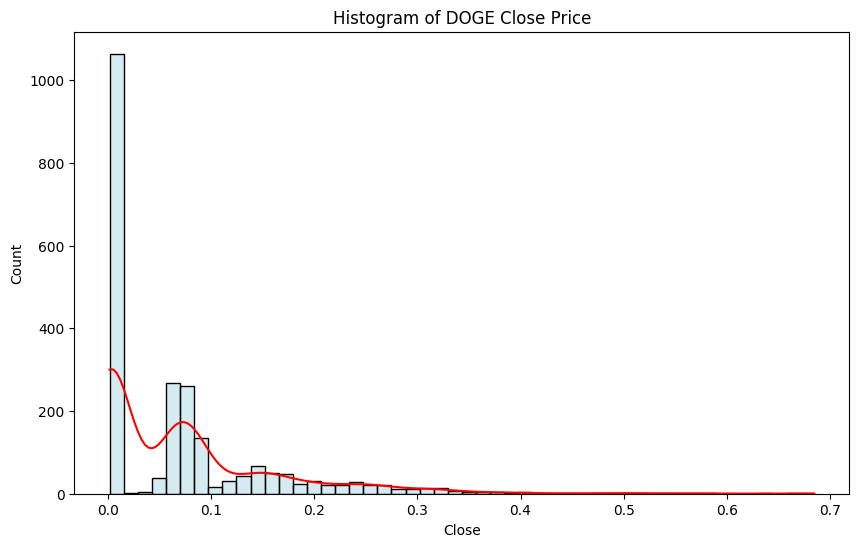
\includegraphics[width=\linewidth]{graph/doge_his.png}
        \caption{DOGE's Histogram}
        \label{fig:2}
    \end{minipage}
\end{figure}

\begin{figure}[H]
    \centering
    \begin{minipage}{0.23\textwidth}
        \centering
        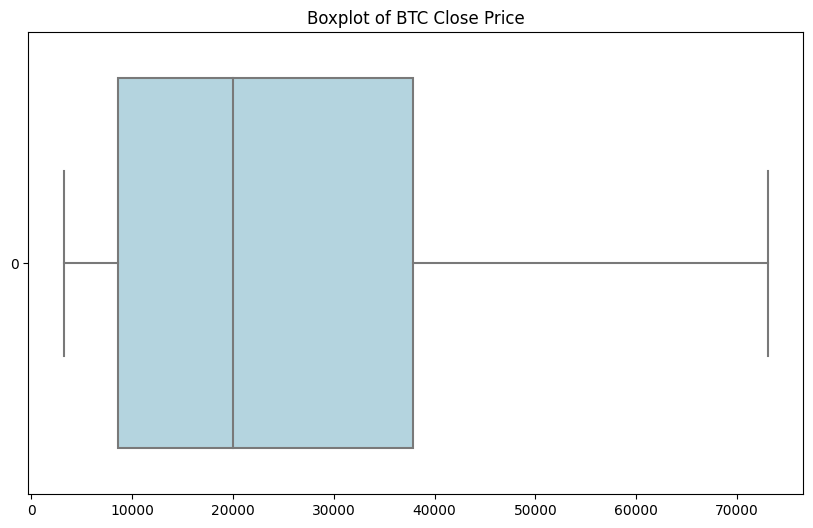
\includegraphics[width=\linewidth]{graph/btc_boxplot.png}
        \caption{BTC's Box Plot}
        \label{fig:3}
    \end{minipage}
    \hfill
    \begin{minipage}{0.23\textwidth}
        \centering
        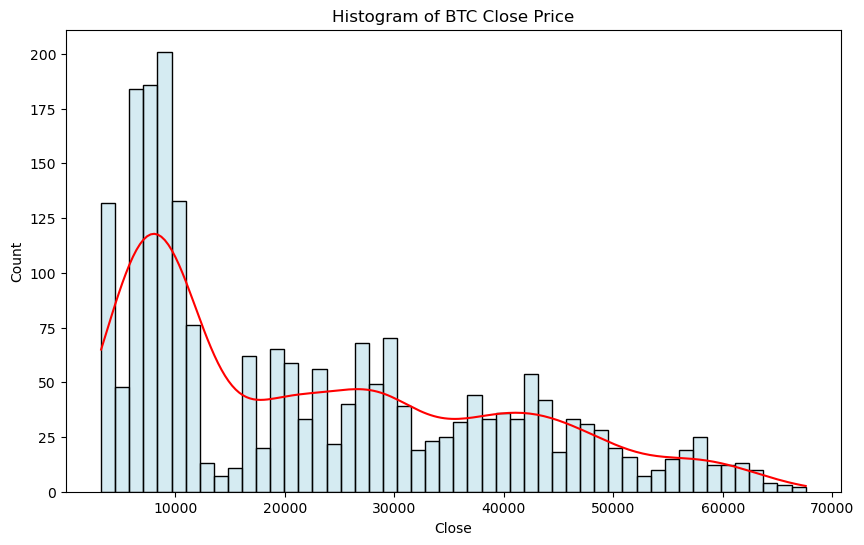
\includegraphics[width=\linewidth]{graph/btc_his.png}
        \caption{BTC's Histogram}
        \label{fig:4}
    \end{minipage}
\end{figure}

\begin{figure}[H]
    \centering
    \begin{minipage}{0.23\textwidth}
        \centering
        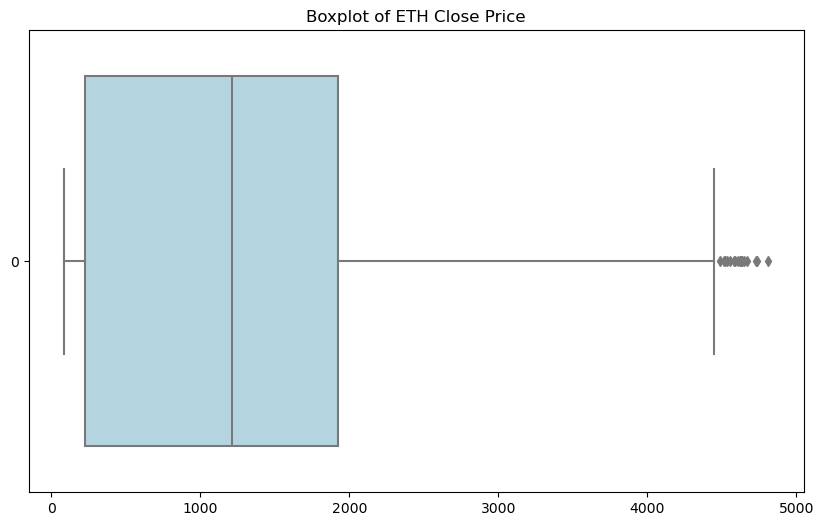
\includegraphics[width=\linewidth]{graph/eth_boxplot.png}
        \caption{ETH's Box Plot}
        \label{fig:5}
    \end{minipage}
    \hfill
    \begin{minipage}{0.23\textwidth}
        \centering
        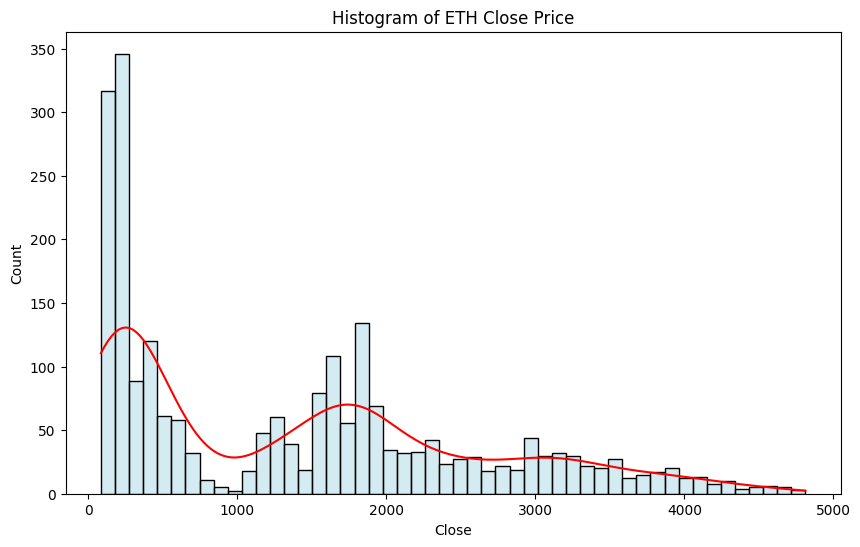
\includegraphics[width=\linewidth]{graph/eth_his.png}
        \caption{ETH's Histogram}
        \label{fig:6}
    \end{minipage}

\end{figure}

\begin{itemize}
    \item Across all three cryptocurrencies, there are remarkable differences in mean values, indicating diverse price levels. Moreover, the considerable range between minimum and maximum values highlights the wide fluctuations in prices, portraying substantial volatility within the market.
    \item The high standard deviation, positive kurtosis, and skewness values suggest non-normal distributions with fat tails and right skewness. This indicates frequent occurrence of outliers and a tendency for prices to be skewed towards higher values, which means the occurrence of high prices isn't significant.
    \item These measures contributes to a summary that it is potential for high profits but also heightened risks when investing in these three cryptocurrencies.

\end{itemize}

\section{Methodology}
\subsection{Linear Regression}
In statistics, Linear Regression is a supervised learning algorithm that simulates a mathematical relationship between a dependent variable and independent
variables, enabling predictions for continuous or numeric variables.\
A multiple linear regression model has the form:
\[Y=\beta_0+\beta_1X_1+\beta_2X_2+\cdots+\beta_kX_k+\varepsilon\]
Where:\\
\indent\textbullet\ Y is the dependent variable (Response variable).\\
\indent\textbullet\ \(X_1, X_2, \ldots, X_k\) are the independent (Explanatory variables).\\
\indent\textbullet\ \(\beta_0\) is the intercept term.\\
\indent\textbullet\ \(\beta_1,..., \beta_k\) are the regression coefficients for the independent variables.\\
\indent\textbullet\ \(\varepsilon\) is the error term.
\subsection{ARIMAX}
\justify
ARIMAX is a time series forecasting model that combines Autoregressive Integrated Moving Average (ARIMA) model with exogenous variables. It extends  ARIMA by  including external  predictors  (denoted as  X) to improve  forecasting accuracy.  This model involves  specifying AR, I,  and MA components,  along with the  exogenous variables, estimating model parameters, and making forecasts \cite{b3}.\\
% ARIMA Models are specified by three order parameters: (p, d, q),\ 

% where,\
%     \indent\textbullet\ p is the order of the AR term
%     \indent\textbullet\ q is the order of the MA term
%     \indent\textbullet\ d is the number of differencing required to make the time series stationary\\

An ARIMAX model depicted by the following equation:
\begin{dmath*}
    Y_t = \alpha
    + \underbrace{\beta_1 X_{1,t} + \ldots + \beta_r X_{r,t}}_{\text{exogenous variables}}
    + \underbrace{\phi_1 Y_{t-1} + \phi_2 Y_{t-2} + \ldots + \phi_p Y_{t-p}}_{\text{AR term}}
    + \underbrace{\varepsilon_t - \theta_1 \varepsilon_{t-1} - \theta_2 \varepsilon_{t-2} - \ldots - \theta_q \varepsilon_{t-q}}_{\text{MA term}}
\end{dmath*}

\subsection{Vector Autoregression}
Vector Autoregression (VAR) is a multivariate forecasting algorithm that is used when two or more time series influence each other. \\
It is considered as a generalization of univariate AR models or a combination between the two or more models and the univariate time series models. Each variable in a VAR is explained by its own lagged values and the lagged values of all the other variables in the equation.The basic VAR (p) model is given by:
\[Y_t=c+A_1y_{t-1}+A_2y_{t-2}+...+A_py_{t-p}+\varepsilon_t\]
Where:\\
\indent\textbullet\ \(y_t-i\): the "ith lag" of \(y_t\)\\
\indent\textbullet\ \(c\) is a k-vector of constants\\
\indent\textbullet\ \(A_i\): time-invariant (k × k)-matrix\\
\indent\textbullet\ \(\boldsymbol{\varepsilon}_t\): a vector of error terms with \(k\) element\\
In matrix form:\\
\begin{dmath*}
    Y_t=\left[\begin{matrix}y_1\\y_2\\\begin{matrix}\begin{matrix}.\\.\\\end{matrix}\\y_k\\\end{matrix}\\\end{matrix}\right]\ =\left[\begin{matrix}c_1\\c_2\\\begin{matrix}\begin{matrix}.\\.\\\end{matrix}\\c_k\\\end{matrix}\\\end{matrix}\right]+\left[\begin{matrix}\begin{matrix}\phi_{11}\\\phi_{21}\\\end{matrix}&\begin{matrix}.\\.\\\end{matrix}&\begin{matrix}.\\.\\\end{matrix}\\\begin{matrix}.\\.\\\end{matrix}&\ &\ \\\phi_{k1}&.&.\\\end{matrix}\right]\left[\begin{matrix}y_{1,t-1}\\y_{2,t-1}\\\begin{matrix}\begin{matrix}.\\.\\\end{matrix}\\y_{k,t-1}\\\end{matrix}\\\end{matrix}\right]+...+\ \left[\begin{matrix}\begin{matrix}\phi_{11}\\\phi_{21}\\\end{matrix}&\begin{matrix}.\\.\\\end{matrix}&\begin{matrix}.\\.\\\end{matrix}\\\begin{matrix}.\\.\\\end{matrix}&\ &\ \\\phi_{k1}&.&.\\\end{matrix}\right]\left[\begin{matrix}y_{1,t-p}\\y_{2,t-p}\\\begin{matrix}\begin{matrix}.\\.\\\end{matrix}\\y_{k,t-p}\\\end{matrix}\\\end{matrix}\right]+\left[\begin{matrix}\varepsilon_1\\\varepsilon_2\\\begin{matrix}\begin{matrix}.\\.\\\end{matrix}\\\varepsilon_k\\\end{matrix}\\\end{matrix}\right]
\end{dmath*}

\subsection{Recurrent Neural Networks (RNN)}
Recurrent Neural Networks (RNNs) are a class of artificial neural networks designed for sequential data, where the connections between nodes form a directed graph along a temporal sequence. This allows RNNs to exhibit temporal dynamic behavior for a time sequence.\ 
\begin{figure}[h]
    \centering
    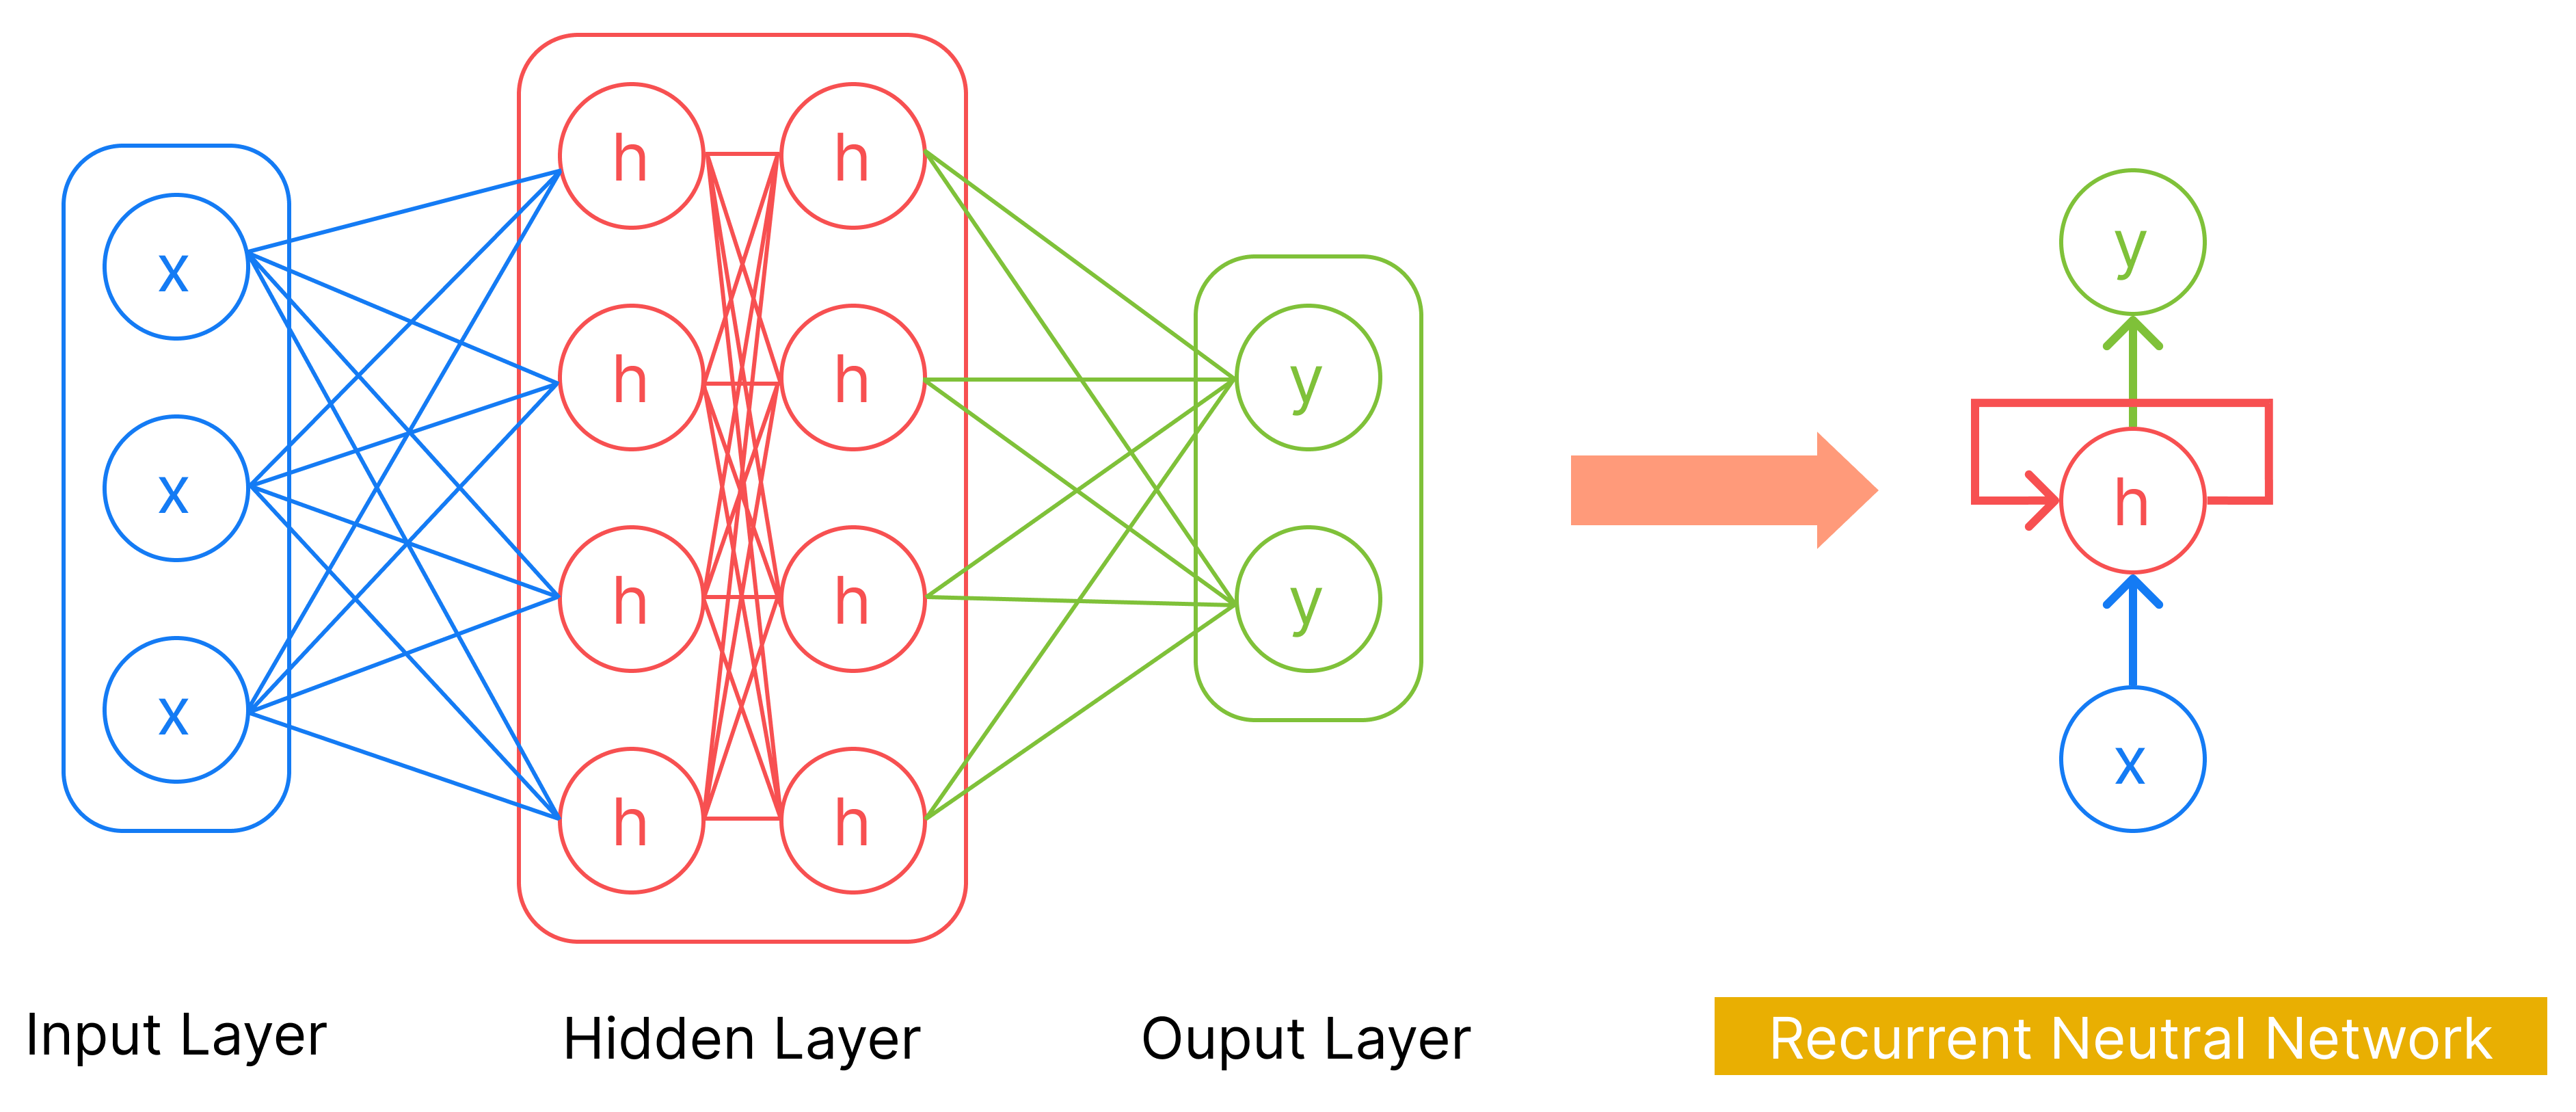
\includegraphics[width=\linewidth]{./image/RNN.png}
    \caption{Model of RNN architectural}
    \label{fig:7}
\end{figure}\\
\begin {itemize}
    \item \textbf{Input Layer}: Networks have only one input layer.
    \item \textbf{Hidden Layer}: Networks have multiple hidden layers.
    \item \textbf{Output Layer}: Networks have only one output layer.
\end {itemize}
A basic RNN can be represented as follows:
\begin{dmath*}
    h_t = f(W_{xh} x_t + W_{hh} h_{t-1} + b_h)
\end{dmath*}
\begin{dmath*}
    y_t = g(W_{hy} h_t + b_y)
\end{dmath*}
Where:\begin {itemize}
\item \(x_t\) is the input at time step \(t\).
\item \(h_t\) is the hidden state at time step \(t\).
\item \(y_t\) is the output at time step \(t\).
\item \(W_{xh}\), \(W_{hh}\), and \(W_{hy}\) are weight matrices.
\item \(b_h\) and \(b_y\) are bias vectors.
\item \(f\) and \(g\) are activation functions.
\end{itemize}

\subsection{Long Short-Term Memory (LSTM)}
Long Short-Term Memory (LSTM) networks are a type of RNN designed to address the vanishing gradient problem that can occur with traditional RNNs when processing long sequences. LSTMs achieve this through a memory cell which is controlled by three gates:\\
\begin{figure}[H]
    \centering
    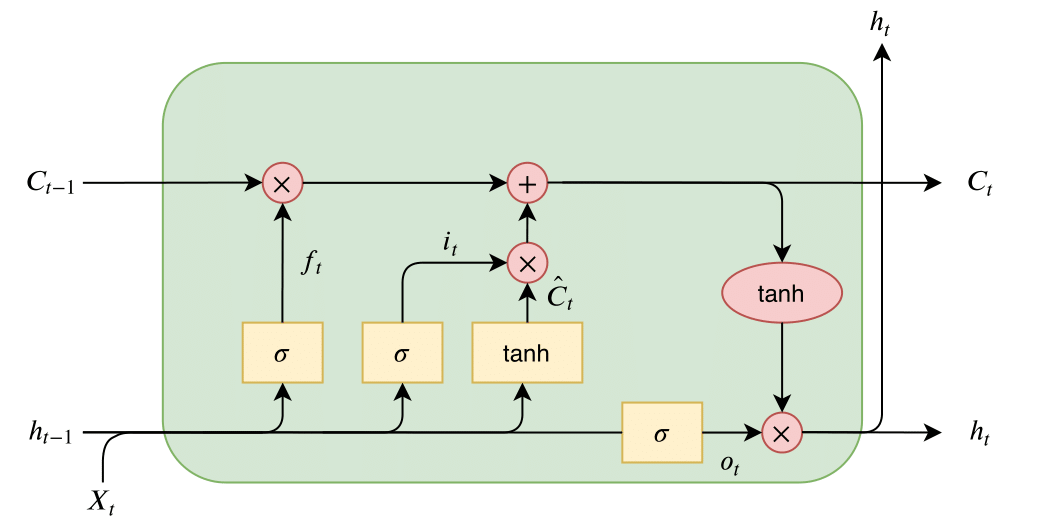
\includegraphics[width=0.8\linewidth]{./image/LSTM.png}
    \caption{Model of LSTM architectural}
    \label{fig:8}
\end{figure}
\noindent
- \textbf{Forget Gate}: Controls what information is discarded from the cell state.
\begin{dmath*}
    f_t = \sigma(W_f \cdot [h_{t-1}, x_t] + b_f)
\end{dmath*}
- \textbf{Input Gate}: Controls what new information is added to the cell state.
\begin{dmath*}
    i_t = \sigma(W_i \cdot [h_{t-1}, x_t] + b_i)
\end{dmath*}
\begin{dmath*}
    \tilde{C}_t = \tanh(W_C \cdot [h_{t-1}, x_t] + b_C)
\end{dmath*}
- \textbf{Output Gate}: Controls what information is output form the cell state.
\begin{dmath*}
    o_t = \sigma(W_o \cdot [h_{t-1}, x_t] + b_o)
\end{dmath*}
Where:
\begin{itemize}
    \item \(W_f\), \(W_i\), \(W_C\), \(W_o\) are the weight matrices of \textbf{f}orget gate, \textbf{i}nput gate, \textbf{C}ell state, and \textbf{o}utput gate respectively.
    \item \(b_f\), \(b_i\), \(b_C\), \(b_o\) are the bias vectors of  \textbf{f}orget gate, \textbf{i}nput gate, \textbf{C}ell state, and \textbf{o}utput gate respectively.
    \item \(\sigma\) is the sigmoid activation function.
    \item \(\tanh\) is tanh activation function that gives an output of vector from -1 to +1.
\end{itemize}
Then the cell state \(C_t\) and hidden state \(h_t\) are then updated as follows:
\begin{dmath*}
    C_t = f_t * C_{t-1} + i_t * \tilde{C}_t
\end{dmath*}
\begin{dmath*}
    h_t = o_t * \tanh(C_t)
\end{dmath*}

\subsection{Gated Recurrent Unit (GRU)}
Gated Recurrent Units (GRUs) are another type of RNN with a simplified gating mechanism compared to LSTMs, which selectively update the hidden state at each time step. The GRU has only two gating mechanisms:\\
\begin{figure}[H]
    \centering
    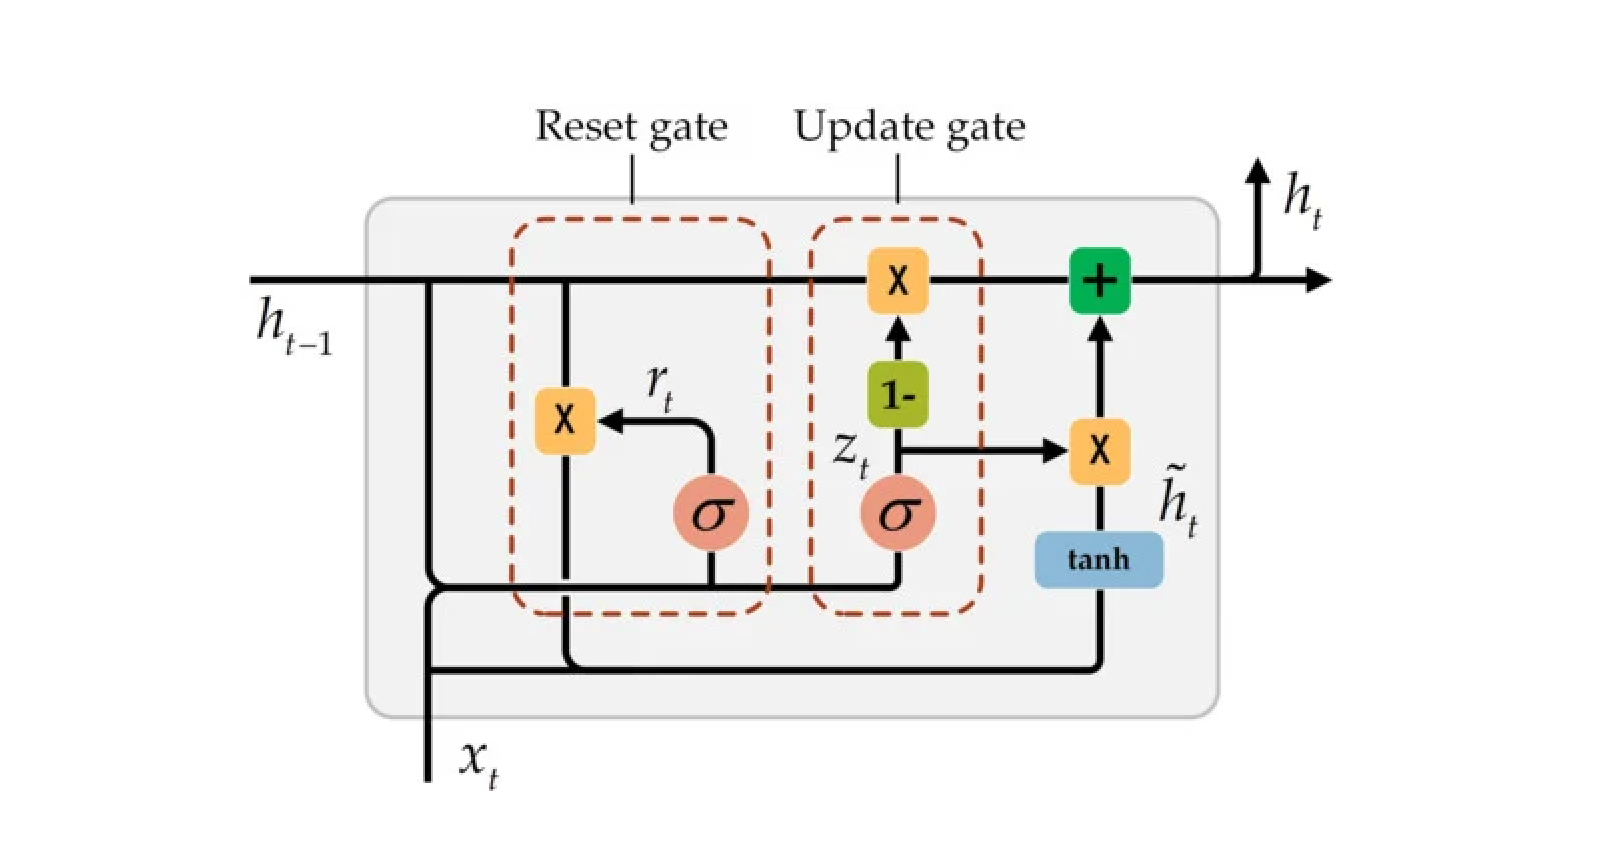
\includegraphics[width=\linewidth]{./image/GRU.png}
    \caption{Model of GRU architectural}
    \label{fig:9}
\end{figure}
\noindent
- \textbf{Update Gate}: Controls the amount of information from the previous hidden state to let through, and the amount of new information to add.
\begin{dmath*}
    z_t = \sigma(W_z \cdot [h_{t-1}, x_t] + b_z)
\end{dmath*}
- \textbf{Reset Gate}: Controls the amount of information to forget from the previous hidden state.
\begin{dmath*}
    r_t = \sigma(W_r \cdot [h_{t-1}, x_t] + b_r)
\end{dmath*}
The candidate hidden state is calculated based on the reset gate and the previous hidden state.
\begin{dmath*}
    \tilde{h}_t = \tanh(W \cdot [r_t * h_{t-1}, x_t] + b)
\end{dmath*}
Then the hidden state is updated based on the update gate and the candidate hidden state.
\begin{dmath*}
    h_t = (1 - z_t) * h_{t-1} + z_t * \tilde{h}_t
\end{dmath*}
Where:
\begin{itemize}
    \item \(z_t\) and \(r_t\) are the update gate and reset gate.
    \item \(W_z\), \(W_r\), \(W\), \(b_z\), \(b_r\), \(b\) are the weight matrices and bias vectors of the update gate, reset gate, and candidate hidden state respectively.
    \item \(\sigma\) is the sigmoid activation function.
    \item \(\tanh\) is the hyperbolic tangent activation function.
\end{itemize}
\subsection{XGBoost}
XGBoost (eXtreme Gradient Boosting) is a powerful machine learning algorithm that uses an ensemble of decision trees and gradient boosting, which combines multiple weak learners to create a strong predictive model, to minimize prediction errors.\\
\begin{figure} [H]
    \centering
    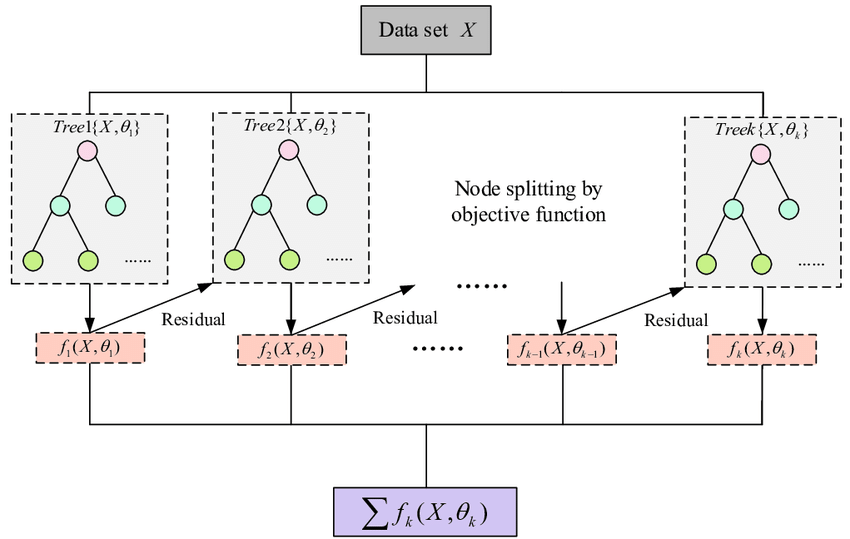
\includegraphics[width=0.8\linewidth]{./image/XGBoost.png}
    \caption{Model of XGBoost architectural}
    \label{fig:10}
\end{figure}
\noindent
- \textbf{Loss Function}: Measures the difference between the true label \(y_i\) and the predicted label \(\hat{y}_i\),\\
\begin{dmath*}
    l(y_i, \hat{y}_i) 
\end{dmath*}
- \textbf{Regularization Term}: Penalizes model complexity to prevent overfitting in each the \(f\) tree.\\
\begin{dmath*}
    \Omega(f) = \gamma T + \frac{1}{2} \lambda ||w||^2
\end{dmath*}
Where:
\begin{itemize}
    \item \(T\) is the number of leaves in the \(f\) tree.
    \item \(w\) is the leaf weight of the \(f\) tree.
    \item \(\lambda\), \(\gamma\)  are the  hyperparameters.
\end{itemize}
- \textbf{Objective Function} = Loss Function + Regularization Term
\begin{dmath*}
    \mathcal{L}(\phi) = \sum_{i=1}^n l(y_i, \hat{y}_i) + \Omega(f_k)
\end{dmath*}
Decision trees are built sequentially to minimize the objective function. At each step, a new tree \(f_t\) with input features \(x_i\) is added to correct the errors of the current model.
\begin{dmath*}
    \hat{y}_i^{(t)} = \hat{y}_i^{(t-1)} + f_t(x_i)
\end{dmath*}
- \textbf{Second-order Taylor expansion} is used to optimized the objective function based on gradient \(g\) and hessian \(h\) of the loss function.
\begin{dmath*}
    \mathcal{L}^{(t)} \approx \sum_{i=1}^n [l(y_i, \hat{y}_i^{(t-1)}) + g_i f_t(x_i) + \frac{1}{2} h_i f_t^2(x_i)] + \Omega(f_t)
\end{dmath*}
Where:
\begin{itemize}
    \item \(n\) is the number of data instances.
    \item \(g_i\) = \(\frac{\partial l(y_i, \hat{y}_i)}{\partial \hat{y}_i}\) and \(h_i\) = \(\frac{\partial^2 l(y_i, \hat{y}_i)}{\partial \hat{y}_i^2}\)
\end{itemize}
And to find the optimal leaf weight \(w_j\) for each leaf node \(j\), the objective function is minimized. Then we have the equation:
\begin{dmath*}
    w_j = -\frac{\sum_{i \in I_j} g_i}{\sum_{i \in I_j} h_i + \lambda}
\end{dmath*}
\subsection{LightGBM}
LightGBM (Light Gradient Boosting Machine) is an advanced machine learning algorithm that builds upon the Gradient Boosting Decision Tree (GBDT) framework. It uses a histogram-based algorithm to speed up training and reduce memory usage.\\
LightGBM grows trees based on leaf-wise, while most other boosting tools (including XGBoost) are based on level-wise. Leaf-wise selects nodes to grow the tree based on optimizing the entire tree, while level-wise optimizes on the branch under consideration. This allows LightGBM to achieve lower loss than other boosting algorithms.
\begin{figure}[H]
    \centering
    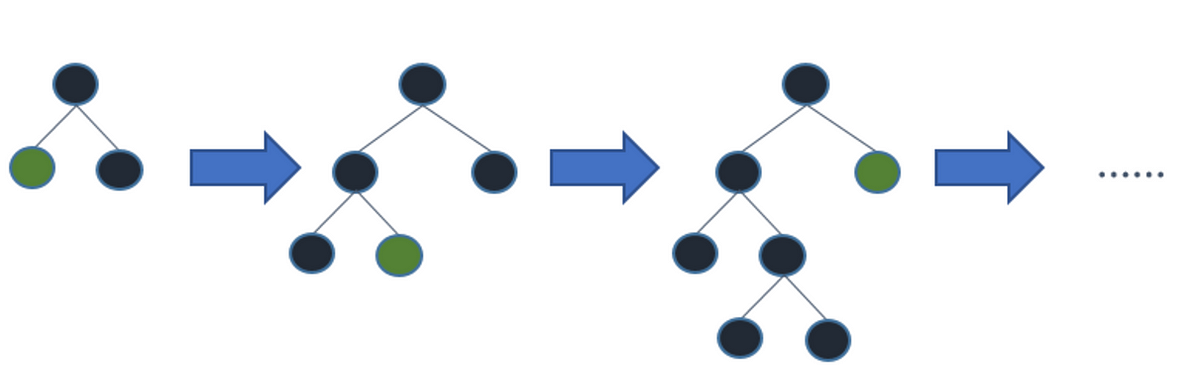
\includegraphics[width=0.8\linewidth]{./image/LightGBM.png}
    \caption{Leaf-wise tree expansion in LightGBM}
    \label{fig:11}
\end{figure}
\noindent
Additionally, LightGBM enhances the efficiency and scalability of GBDT through the integration of two novel techniques: Gradient-based One-Side Sampling (GOSS) and Exclusive Feature Bundling (EFB) \cite{b9}.\\
%- \textbf{GOSS}: Retains all instances with large gradients and samples a subset of instances with small gradients to reduce the number of instances.\\
%- \textbf{EFB}: Bundles exclusive features to reduce the number of features and improve efficiency.\\
\begin{itemize}
    \item \textbf{Gradient-based One-Side Sampling (GOSS)}\\
    %GOSS keeps all the instances with large gradients and performs random sampling on the instanceswith small gradients. In order to compensate the influence to the data distribution, when computing theinformation gain, GOSS introduces a constant multiplier for the data instances with small gradients(see Alg. 2). Specifically, GOSS firstly sorts the data instances according to the absolute value of theirgradients and selects the topa×100%instances. Then it randomly samplesb×100%instances fromthe rest of the data. After that, GOSS amplifies the sampled data with small gradients by a constant1−abwhen calculating the information gain. By doing so, we put more focus on the under-trainedinstances without changing the original data distribution by much.
    GOSS keeps all the instances with large gradients and performs random sampling on the instances with small gradients. In order to compensate for the influence on the data distribution, when computing the information gain, GOSS introduces a constant multiplier for the data instances with small gradients. Specifically, GOSS first sorts the data instances according to the absolute value of their gradients and selects the top \(a \times 100\%\) instances. Then it randomly samples \(b \times 100\%\) instances from the rest of the data. After that, GOSS amplifies the sampled data with small gradients by a constant \(\frac{1-a}{b}\) when calculating the information gain.\\
    %By doing so, we put more focus on the under-trained instances without changing the original data distribution by much.
    \item \textbf{Exclusive Feature Bundling (EFB)}\\
    High-dimensional data often have many features, but most of them are sparse, meaning they frequently take on zero values. Because many features are mutually exclusive (never nonzero at the same time), we can combine these features into Exclusive Feature Bundles. By a carefully designed feature scanning algorithm, we can build thesame feature histograms from the feature bundles as those from individual features. In this way, thecomplexity of histogram building changes from \(O(\#data \times \#feature)\) to \(O(\#data \times \#bundle)\), while \#bundle << \#feature. %This can greatly reduce the time and memory consumption of histogram building. 
\end{itemize}
However,  LightGBM  regression  has  disadvantages in generating the overfitting model as well as being sensitive the noise.

\section{Experiment}
\subsection{Feature Engineering}
In this section, we focus on constructing diverse input features derived from technical indicators related to the Close price only. These features aim to enhance the predictive capabilities of our models and support continuous forecasting for out-of-sample (OOS) data. The selected indicators include the Moving Average Convergence/Divergence (MACD), Bollinger Bands (Upper and Lower), 26-period Moving Average (\(MA_{26}\)), and 20-period Exponential Moving Average (\(EMA_{20}\)).\\ 
MACD: The MACD is a trend-following momentum indicator that shows the relationship between two moving averages of a security’s price. It is calculated by subtracting the 26-period EMA from the 12-period EMA. The MACD helps identify changes in the strength, direction, momentum, and duration of a trend in a security’s price.
\begin{dmath*}
    MACD = EMA_{12} - EMA_{26}
\end{dmath*}
Bollinger Band (BBand): BBands consist of a middle band (20-period moving average) and two outer bands (standard deviations away from the middle band). The upper and lower bands provide a relative definition of high and low prices. The upper BBand is calculated by adding two standard deviations to the 20-period moving average, and the lower BBand is calculated by subtracting two standard deviations from the 20-period moving average
\begin{dmath*}
    Upper Band = MA_{20} + (2 \times \text{Standard Deviation})
\end{dmath*}
\begin{dmath*}
    Lower Band = MA_{20} - (2 \times \text{Standard Deviation})
\end{dmath*}
\noindent
\(MA_{26}\): The \(MA_{26}\) is a simple moving average calculated by averaging the closing prices over the last 26 periods. It helps smooth out price data to identify the direction of the trend over a medium-term period.
\begin{dmath*}
    MA_{26} = \frac{1}{26} \sum_{i=1}^{26} \text{Close}_i
\end{dmath*}
\noindent
\(EMA_{20}\): The \(EMA_{20}\) is a type of moving average that places a greater weight and significance on the most recent data points. The EMA20 responds more quickly to recent price changes compared to the simple moving average. It is used to identify short-term trends.
\begin{dmath*}
    %EMA_20 = \frac{2}{21} \times \text{Close} + \frac{19}{21} \times \text{EMA}_{19}
    EMA_{20} = (Close_t \times \frac{2}{1+20}) + (EMA_{20,t-1} \times (1-\frac{2}{20+1}))
\end{dmath*}
\subsection {Dataset Split Ratio}
The dataset is divided into training and testing sets with three ratios of 70:30, 80:20, and 90:10. The training set is used to train the model, while the testing set is used to evaluate the model's performance.\\
To improve the dataset, we will use the following preprocessing techniques: data cleansing, feature selection.
\subsection {Evaluation Methods}
This paper uses three metrics to evaluate the performance of the models: Root Mean Squared Error (RMSE) Mean Absolute Percentage Error (MAPE) and Symmetric Mean Absolute Percentage Error (SMAPE)\\
%formula
With:
\begin{itemize}
    \item \(y_i\): Actual value
    \item \(\hat{y}_i\): Predicted value
    \item \(n\): Number of data points
\end{itemize}
\noindent
- \textbf{Root Mean Squared Error (RMSE)}: Measures the average of the squared differences between the predicted and actual values.
    \begin{dmath*}
        RMSE = \sqrt{\frac{1}{n} \sum_{i=1}^{n} (y_i - \hat{y}_i)^2}
    \end{dmath*}
    (Best value = 0, Worst value = \(+\infty\))\\
\noindent
- \textbf{Mean Absolute Percentage Error (MAPE)}: Measures the average of the absolute percentage differences between the predicted and actual values.
    \begin{dmath*}
        MAPE = \frac{1}{n} \sum_{i=1}^{n} \left| \frac{y_i - \hat{y}_i}{y_i} \right| \times 100
    \end{dmath*}
        (Best value = 0, Worst value = \(+\infty\%\))\\
\noindent
- \textbf{Symmetric Mean Absolute Percentage Error (SMAPE)}: Measures the symmetric average of the absolute percentage differences between the predicted and actual values.
    \begin{dmath*}
        SMAPE = \frac{1}{n} \sum_{i=1}^{n} \frac{\left| y_i - \hat{y}_i \right|}{\left( \left| y_i \right| + \left| \hat{y}_i \right| \right)/2} \times 100
    \end{dmath*}
    (Best value = 0, Worst value = 200\%)\\
\subsection {Results}
\begin{table}[H]
    \begin{tabular*}{\linewidth}{@{\extracolsep{\fill}}|c|c|c|c|c|}
        \hline
        \textbf{Model} & \textbf{Ratio} & \textbf{RMSE} & \textbf{MAPE} & \textbf{SMAPE} \\
        \hline
        % 1.486,62	2,88	2,91	bold 1.684,85	bold 2,66	bold 2,69	2.171,14	2,89	2,91
        Linear Regression & \makecell{7:3 \\ \textbf{8:2} \\ 9:1} & \makecell{1.486,62 \\ \textbf{1.684,85} \\ 2.171,14} & \makecell{2,88 \\ \textbf{2,66} \\ 2,89} & \makecell{2,91 \\ \textbf{2,69} \\ 2,91} \\
        \hline
        % 16.983,58	29,76	37,00	bold 11.725,95	bold 16,94	bold 18,74	15.950,28	21,44	25,09
        ARIMAX & \makecell{7:3 \\ \textbf{8:2} \\ 9:1} & \makecell{16.983,58 \\ \textbf{11.725,95} \\ 15.950,28} & \makecell{29,76 \\ \textbf{16,94} \\ 21,44} & \makecell{37,00 \\ \textbf{18,74} \\ 25,09} \\
        \hline
        %20.608,81	34,19	44,80	bold 1438,.54	22,80	24,58	18.135,05	23,62	28,40
        VAR & \makecell{7:3 \\ \textbf{8:2} \\ 9:1} & \makecell{20.608,81 \\ \textbf{1438,54} \\ 18.135,05} & \makecell{34,19 \\ \textbf{22,80} \\ 23,62} & \makecell{44,80 \\ \textbf{24,58} \\ 28,40} \\
        \hline
        % 1.640,65	3,27	3,33	bold 1.514,22	2,17	2,18	2.009,36	2,62	2,66
        RNN & \makecell{7:3 \\ \textbf{8:2} \\ 9:1} & \makecell{1.640,65 \\ \textbf{1.514,22} \\ 2.009,36} & \makecell{3,27 \\ \textbf{2,17} \\ 2,62} & \makecell{3,33 \\ \textbf{2,18} \\ 2,66} \\
        \hline
        %1.629,24	2,93	2,97	1.584,69	3,27	3,21	bold 1.782,90	2,46	2,45
        LSTM & \makecell{7:3 \\ 8:2 \\ \textbf{9:1}} & \makecell{1.629,24 \\ 1.584,69 \\ \textbf{1.782,90}} & \makecell{2,93 \\ 3,27 \\ \textbf{2,46}} & \makecell{2,97 \\ 3,21 \\ \textbf{2,45}} \\
        \hline
        % bold 1.142,67	1,96	1,95	1.363,21	2,53	2,50	1659,08	2,12	2,12
        GRU & \makecell{\textbf{7:3} \\ 8:2 \\ 9:1} & \makecell{\textbf{1.142,67} \\ 1.363,21 \\ 1.659,08} & \makecell{\textbf{1,96} \\ 2,53 \\ 2,12} & \makecell{\textbf{1,95} \\ 2,50 \\ 2,12} \\
        \hline
        %3.553,40	8,20	8,46	3.630,37	6,43	6,70	bold 4.502,40	6,30	6,30
        XGBoost & \makecell{7:3 \\ 8:2 \\ \textbf{9:1}} & \makecell{3.553,40 \\ 3.630,37 \\ \textbf{4.502,40}} & \makecell{8,20 \\ 6,43 \\ \textbf{6,30}} & \makecell{8,46 \\ 6,70 \\ \textbf{6,30}} \\
        \hline
        %bold 3.172,67	5,88	5,92	4.251,13	8,97	9,52	4.757,29	6,35	6,57
        LightGBM & \makecell{\textbf{7:3} \\ 8:2 \\ 9:1} & \makecell{\textbf{3.172,67} \\ 4.251,13 \\ 4.757,29} & \makecell{\textbf{5,88} \\ 8,97 \\ 6,35} & \makecell{\textbf{5,92} \\ 9,52 \\ 6,57} \\
        \hline
    \end{tabular*}
    \caption{BTC Dataset}
    \label{table:2}
\end{table}
Based on the result table above, we can see that the GRU model is the best-performing model among the 8 implemented models in predicting BTC stock prices with a 7:3 ratio, as it has the lowest RMSE, MAPE, and SMAPE values.
\begin{table}[H]
    \begin{tabular*}{\linewidth}{@{\extracolsep{\fill}}|c|c|c|c|c|}
        \hline
        \textbf{Model} & \textbf{Ratio} & \textbf{RMSE} & \textbf{MAPE} & \textbf{SMAPE} \\
        \hline
        %101,12	3,28	3,31	bold 111,42	bold 3,01	bold 3,03	147,02	3,66	3,68
        Linear Regression & \makecell{7:3 \\ \textbf{8:2} \\ 9:1} & \makecell{101,12 \\ \textbf{111,42} \\ 147,02} & \makecell{3,28 \\ \textbf{3,01} \\ 3,66} & \makecell{3,31 \\ \textbf{3,03} \\ 3,68} \\
        \hline
        %680,62	21,78	25,41	bold 475,30	14,22	14,69	745,42	20,44	23,37v
        ARIMAX & \makecell{7:3 \\ \textbf{8:2} \\ 9:1} & \makecell{680,62 \\ \textbf{475,30} \\ 745,42} & \makecell{21,78 \\ \textbf{14,22} \\ 20,44} & \makecell{25,41 \\ \textbf{14,69} \\ 23,37} \\
        \hline
        %729,78	19,41	22,73	bold 575,95	19,87	19,47	1.047,97	28,03	34,15
        VAR & \makecell{7:3 \\ \textbf{8:2} \\ 9:1} & \makecell{729,78 \\ \textbf{575,95} \\ 1.047,97} & \makecell{19,41 \\ \textbf{19,87} \\ 28,03} & \makecell{22,73 \\ \textbf{19,47} \\ 34,15} \\
        \hline
        % 127,70	5,81	6,01	170,59	7,43	7,13	bold 151,67	4,62	4,77
        RNN & \makecell{7:3 \\ 8:2 \\ \textbf{9:1}} & \makecell{127,70 \\ 170,59 \\ \textbf{151,67}} & \makecell{5,81 \\ 7,43 \\ \textbf{4,62}} & \makecell{6,01 \\ 7,13 \\ \textbf{4,77}} \\
        \hline
        %79,93	2,56	2,52	bold 81,12	2,13	2,16	108,02	2,71	2,71
        LSTM & \makecell{7:3 \\ \textbf{8:2} \\ 9:1} & \makecell{79,93 \\ \textbf{81,12} \\ 108,02} & \makecell{2,56 \\ \textbf{2,13} \\ 2,71} & \makecell{2,52 \\ \textbf{2,16} \\ 2,71} \\
        \hline
        %102,98	4,27	4,13	bold 92,33	3,02	2,97	109,55	2,70	2,74
        GRU & \makecell{7:3 \\ \textbf{8:2} \\ 9:1} & \makecell{102,98 \\ \textbf{92,33} \\ 109,55} & \makecell{4,27 \\ \textbf{3,02} \\ 2,70} & \makecell{4,13 \\ \textbf{2,97} \\ 2,74} \\
        \hline
        %143,88	5,54	5,35	bold 144,28	3,98	3,95	175,47	4,58	4,61
        XGBoost & \makecell{7:3 \\ \textbf{8:2} \\ 9:1} & \makecell{143,88 \\ \textbf{144,28} \\ 175,47} & \makecell{5,54 \\ \textbf{3,98} \\ 4,58} & \makecell{5,35 \\ \textbf{3,95} \\ 4,61} \\
        \hline
        LightGBM & \makecell{7:3 \\ \textbf{8:2} \\ 9:1} & \makecell{130,99 \\ \textbf{137,65} \\ 183,24} & \makecell{5,13 \\ \textbf{4,23} \\ 5,10} & \makecell{4,97 \\ \textbf{4,21} \\ 5,12} \\
        \hline
    \end{tabular*}
% \end{table}
    
% \begin{table}[H]
%     \centering
%     \begin{tabular*}{\linewidth}{@{\extracolsep{\fill}}|m{2cm}|c|c|c|c|}
%         \hline
%         %130,99	5,13	4,97	137,65	4,23	4,21	183,24	5,10	5,12
%         LightGBM & \makecell{7:3 \\ 8:2 \\ 9:1} & \makecell{130,99 \\ 137,65 \\ 183,24} & \makecell{5,13 \\ 4,23 \\ 5,10} & \makecell{4,97 \\ 4,21 \\ 5,12} \\
%         \hline
%     %ETH Dâtaset
    % \end{tabular*}
    \caption{ETH Dataset}
    \label{table:3}
\end{table}
%min value of rmse, mape, smape is model? at ratio? 
Based on the result table above, we can see that the LSTM model is the best-performing model among the 8 implemented models in predicting ETH stock prices with a 8:2 ratio, as it has the lowest RMSE, MAPE, and SMAPE values.
\begin{table}[H]
    \begin{tabular*}{\linewidth}{@{\extracolsep{\fill}}|c|c|c|c|c|}
        \hline
        \textbf{Model} & \textbf{Ratio} & \textbf{RMSE} & \textbf{MAPE} & \textbf{SMAPE} \\
        \hline
        %0,01	4,62	4,69	bold 0,01	bold 3,99	bold 4,04	0,01	5,13	5,23
        Linear Regression & \makecell{7:3 \\ \textbf{8:2} \\ 9:1} & \makecell{0,01 \\ \textbf{0,01} \\ 0,01} & \makecell{4,62 \\ \textbf{3,99} \\ 5,13} & \makecell{4,69 \\ \textbf{4,04} \\ 5,23} \\
        \hline
        %0,0524	31,25	41,65	bold 0,0487	32,24	34,58	0,0757	39,69	56,11
        ARIMAX & \makecell{7:3 \\ \textbf{8:2} \\ 9:1} & \makecell{0,0524 \\ \textbf{0,0487} \\ 0,0757} & \makecell{31,25 \\ \textbf{32,24} \\ 39,69} & \makecell{41,65 \\ \textbf{34,58} \\ 56,11} \\
        \hline
        %bold 0,03	18,42	21,21	0,04	32,18	29,94	0,06	29,87	38,82
        VAR & \makecell{\textbf{7:3} \\ 8:2 \\ 9:1} & \makecell{\textbf{0,03} \\ 0,04 \\ 0,06} & \makecell{\textbf{18,42} \\ 32,18 \\ 29,87} & \makecell{\textbf{21,21} \\ 29,94 \\ 38,82} \\
        \hline
        %0,0081	6,93	6,65	0,0097	9,36	9,82	bold 0,0111	6,35	6,38
        RNN & \makecell{7:3 \\ 8:2 \\ \textbf{9:1}} & \makecell{0,0081 \\ 0,0097 \\ \textbf{0,0111}} & \makecell{6,93 \\ 9,36 \\ \textbf{6,35}} & \makecell{6,65 \\ 9,82 \\ \textbf{6,38}} \\
        \hline
        %0,01	11,12	11,88	0,01	11,03	11,77	bold 0,01	4,51	4,45
        LSTM & \makecell{7:3 \\ 8:2 \\ \textbf{9:1}} & \makecell{0,01 \\ 0,01 \\ \textbf{0,01}} & \makecell{11,12 \\ 11,03 \\ \textbf{4,51}} & \makecell{11,88 \\ 11,77 \\ \textbf{4,45}} \\
        \hline
        %bold 0,0067	5,50	5,64	0,0096	9,00	8,56	0,0081	4,17	4,12
        GRU & \makecell{\textbf{7:3} \\ 8:2 \\ 9:1} & \makecell{\textbf{0,0067} \\ 0,0096 \\ 0,0081} & \makecell{\textbf{5,50} \\ 9,00 \\ 4,17} & \makecell{\textbf{5,64} \\ 8,56 \\ 4,12} \\
        \hline
        %0,02	10,13	9,85	bold 0,02	6,95	7,21	0,02	10,68	11,41
        XGBoost &  \makecell{7:3 \\ \textbf{8:2} \\ 9:1} & \makecell{0,02 \\ \textbf{0,02} \\ 0,02} & \makecell{10,13 \\ \textbf{6,95} \\ 10,68} & \makecell{9,85 \\ \textbf{7,21} \\ 11,41} \\
        \hline
        %0,0134	9,26	9,01	bold 0,02	8,81	8,03	0,0300	12,90	11,43
        LightGBM & \makecell{7:3 \\ \textbf{8:2} \\ 9:1} & \makecell{0,0134 \\ \textbf{0,02} \\ 0,0300} & \makecell{9,26 \\ \textbf{8,81} \\ 12,90} & \makecell{9,01 \\ \textbf{8,03} \\ 11,43} \\
        \hline
    \end{tabular*}
    \caption{DOGE Dataset}
    \label{table:4}
\end{table}
%min value of rmse, mape, smape is model? at ratio?
Based on the result table above, we can see that the GRU model is the best-performing model among the 8 implemented models in predicting DOGE stock prices with a 9:1 ratio, as it has the lowest RMSE, MAPE, and SMAPE values.
\subsection{Visualize}
% %30,60,90 days predict
% Visualizing the predicted and actual values of the BTC dataset using the GRU model with a 7:3 ratio for 30, 60, and 90 days.
% \begin{figure}[H]
%     \centering
%     \includegraphics[width=0.8\linewidth]{./graph/BTC-GRU-70-30.png}
%     \caption{Prediction of BTC using the GRU model with a 7:3 ratio}
%     \label{fig:12}
% \end{figure}
% %30,60,90 days predict, ETH dataset, LSTM model, 8:2 ratio
% Visualizing the predicted and actual values of the ETH dataset using the LSTM model with an 8:2 ratio for 30, 60, and 90 days.
% \begin{figure}[H]
%     \centering
%     \includegraphics[width=0.8\linewidth]{./graph/ETH-LSTM-80-20.png}
%     \caption{Prediction of ETH using the LSTM model with an 8:2 ratio}
%     \label{fig:13}
% \end{figure}
% %30,60,90 days predict, DOGE dataset, GRU model, 7:3 ratio
% Visualizing the predicted and actual values of the DOGE dataset using the GRU model with a 7:3 ratio for 30, 60, and 90 days.
% \begin{figure}[H]
%     \centering
%     \includegraphics[width=0.8\linewidth]{./graph/DOGE-GRU-70-30.png}
%     \caption{Prediction of DOGE using the GRU model with a 7:3 ratio}
%     \label{fig:14}
% \end{figure}
\subsubsection{BTC Dataset}
\begin{figure}[H]
    \centering 
    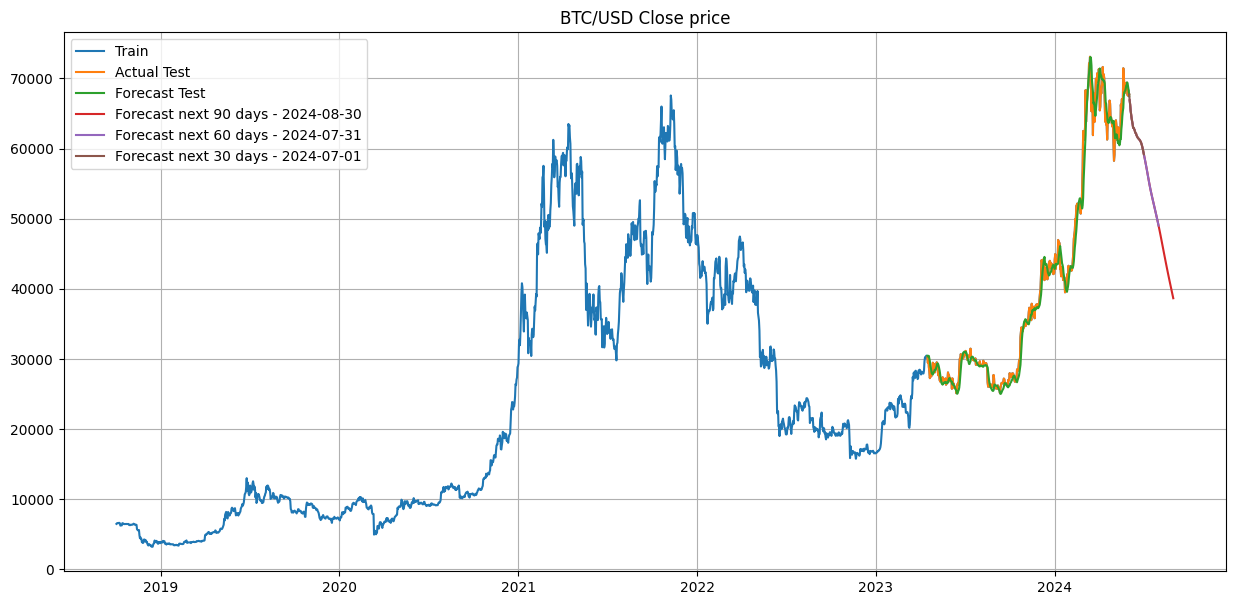
\includegraphics[width=0.8\linewidth]{./././visualize/LinearRegression/BTC-80-20.png} 
    \caption{Linear Regression model’s result with 8:2 ratio}
    \label{fig:12}
\end{figure}
\begin{figure}[H]
    \centering 
    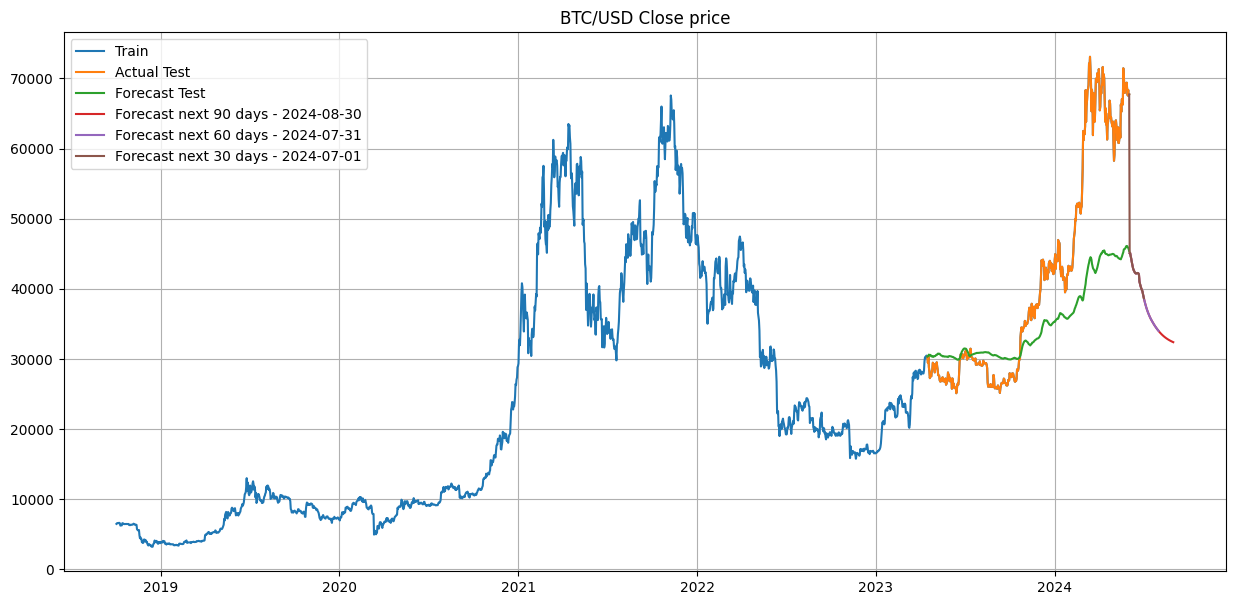
\includegraphics[width=0.8\linewidth]{./././visualize/ARIMAX/BTC-80-20.png} 
    \caption{ARIMAX model’s result with 8:2 ratio}
    \label{fig:13}
\end{figure}
\begin{figure}[H]
    \centering 
    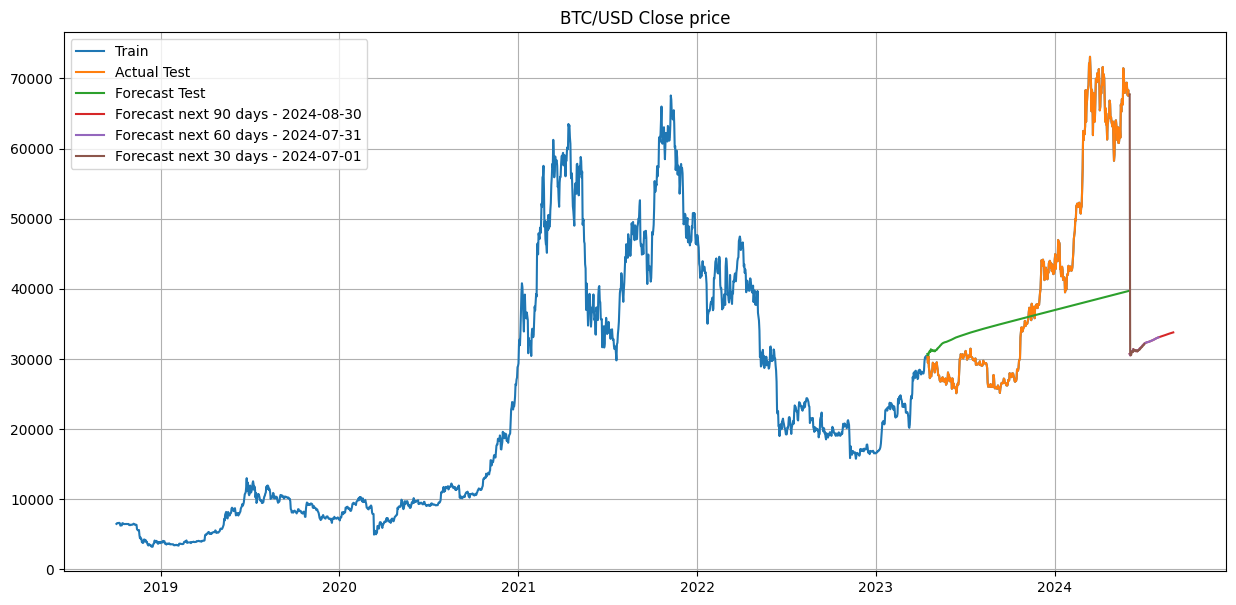
\includegraphics[width=0.8\linewidth]{./././visualize/VAR/BTC-80-20.png} 
    \caption{VAR model’s result with 8:2 ratio}
    \label{fig:14}
\end{figure}
\begin{figure}[H]
    \centering 
    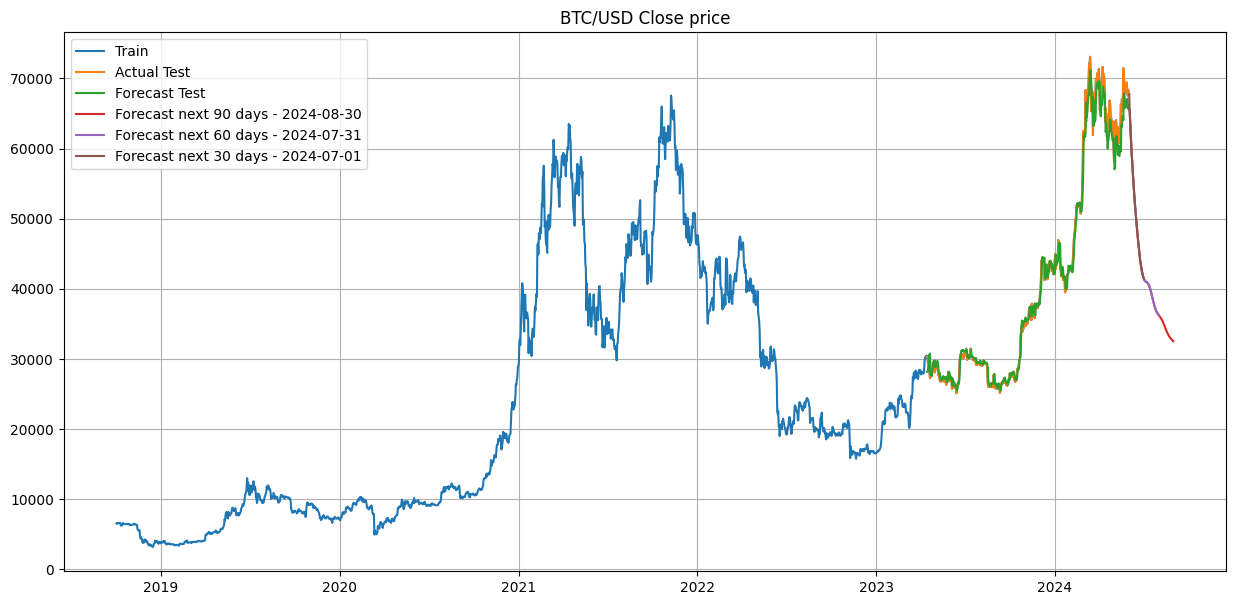
\includegraphics[width=0.8\linewidth]{./././visualize/RNN/BTC-80-20.png} 
    \caption{RNN model’s result with 8:2 ratio}
    \label{fig:15}
\end{figure}
\begin{figure}[H]
    \centering 
    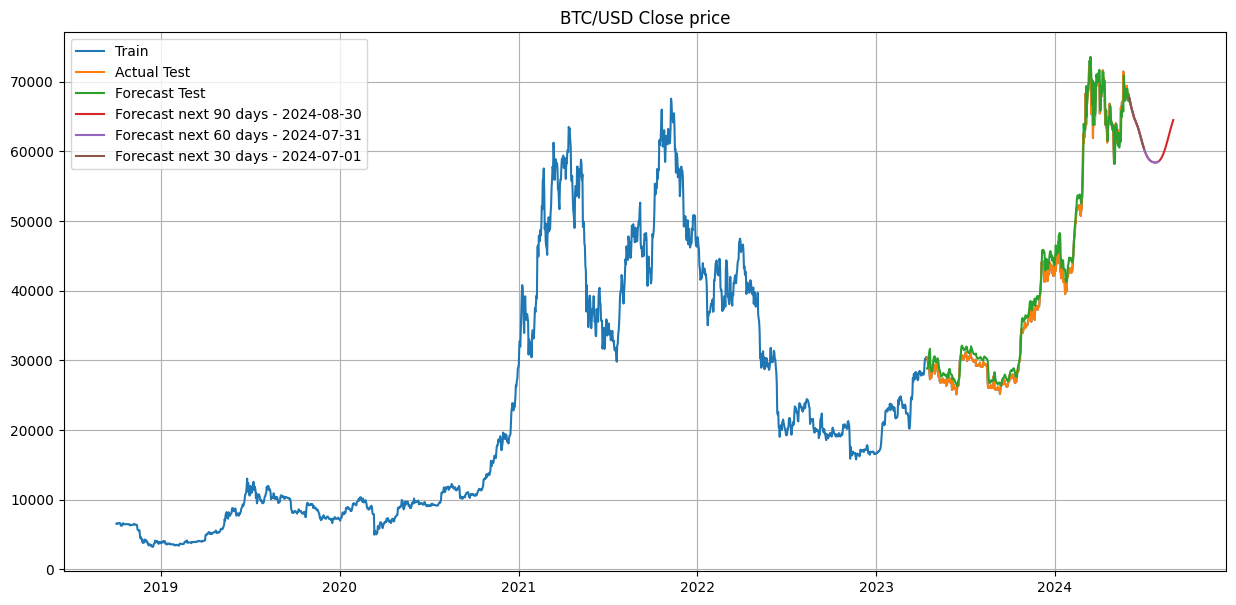
\includegraphics[width=0.8\linewidth]{./././visualize/LSTM/BTC-80-20.png} 
    \caption{LSTM model’s result with 8:2 ratio}
    \label{fig:16}
\end{figure}
%lstm 9:1
\begin{figure}[H]
    \centering 
    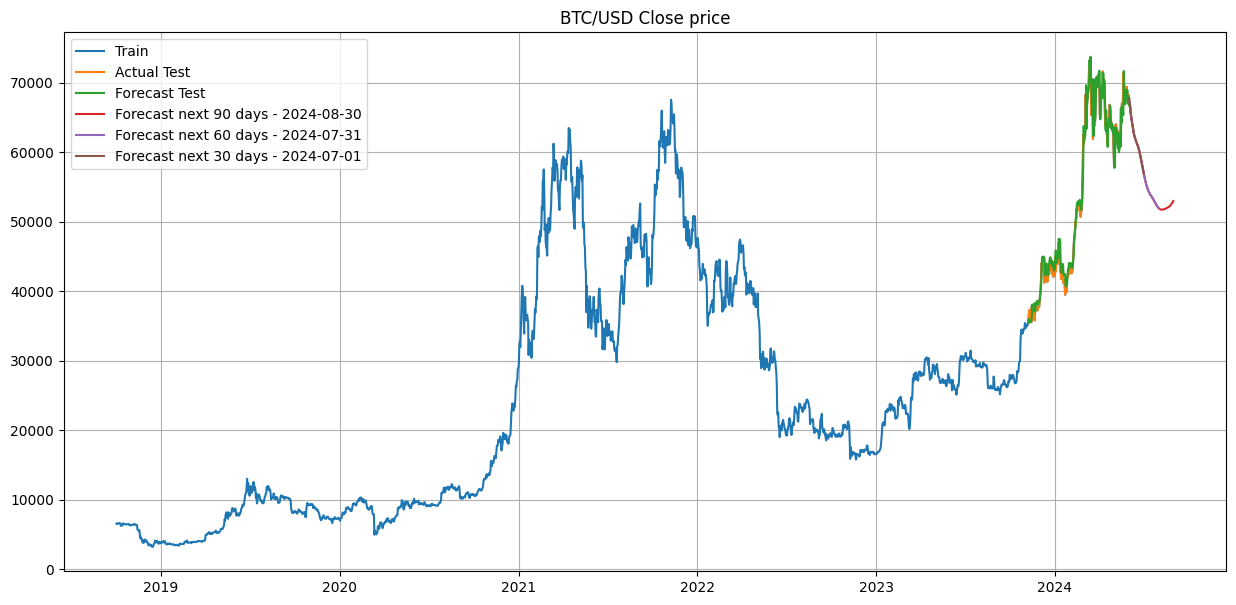
\includegraphics[width=0.8\linewidth]{./././visualize/LSTM/BTC-90-10.png} 
    \caption{LSTM model’s result with 9:1 ratio}
    \label{fig:17}
\end{figure}

%xgboost 9:1
\begin{figure}[H]
    \centering 
    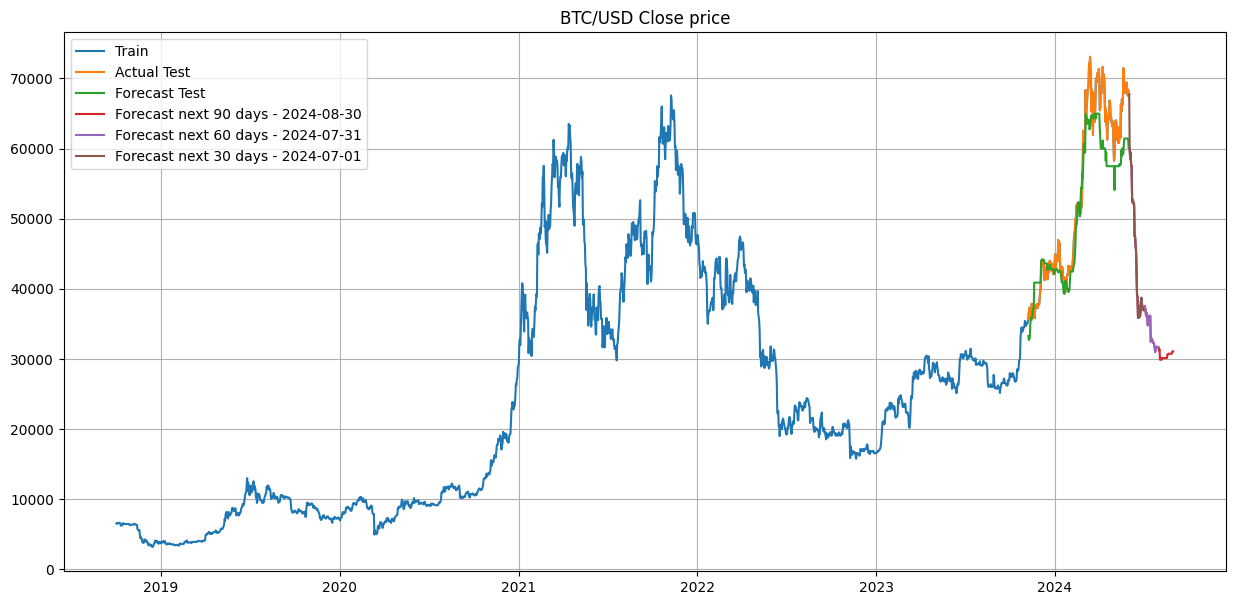
\includegraphics[width=0.8\linewidth]{./././visualize/XGBoost/BTC-90-10.png} 
    \caption{XGBoost model’s result with 9:1 ratio}
    \label{fig:19}
\end{figure}
%lightgbm 7:3
\begin{figure}[H]
    \centering 
    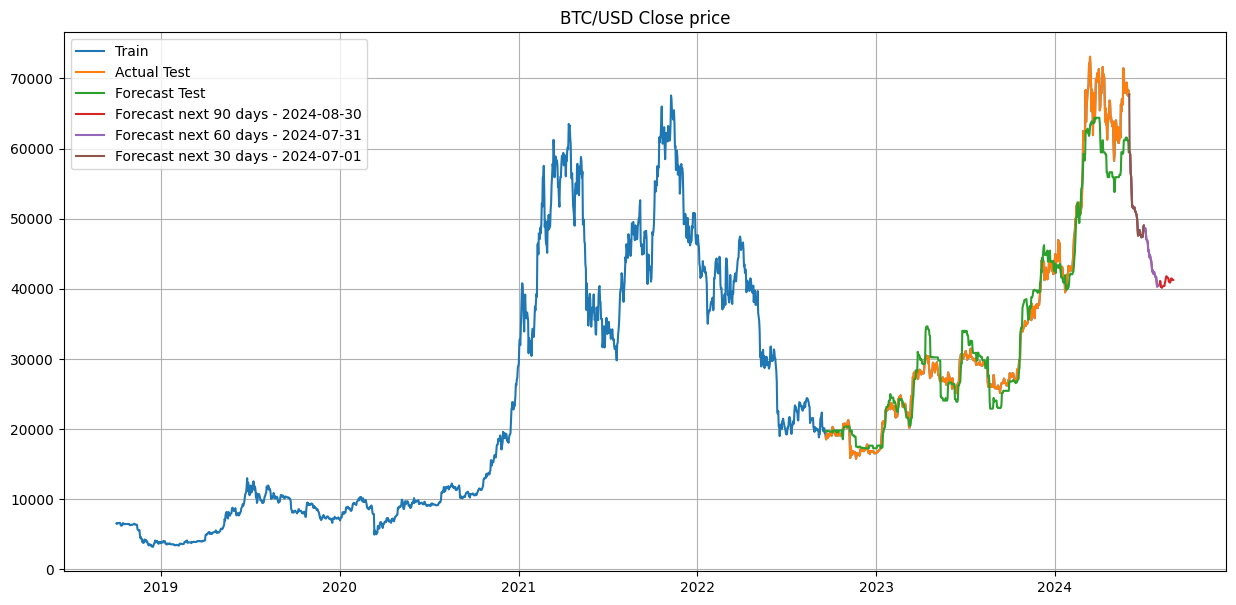
\includegraphics[width=0.8\linewidth]{./././visualize/LightGBM/BTC-70-30.png} 
    \caption{LightGBM model’s result with 7:3 ratio}
    \label{fig:20}
\end{figure}
\subsubsection{ETH Dataset}
\begin{figure}[H]
    \centering 
    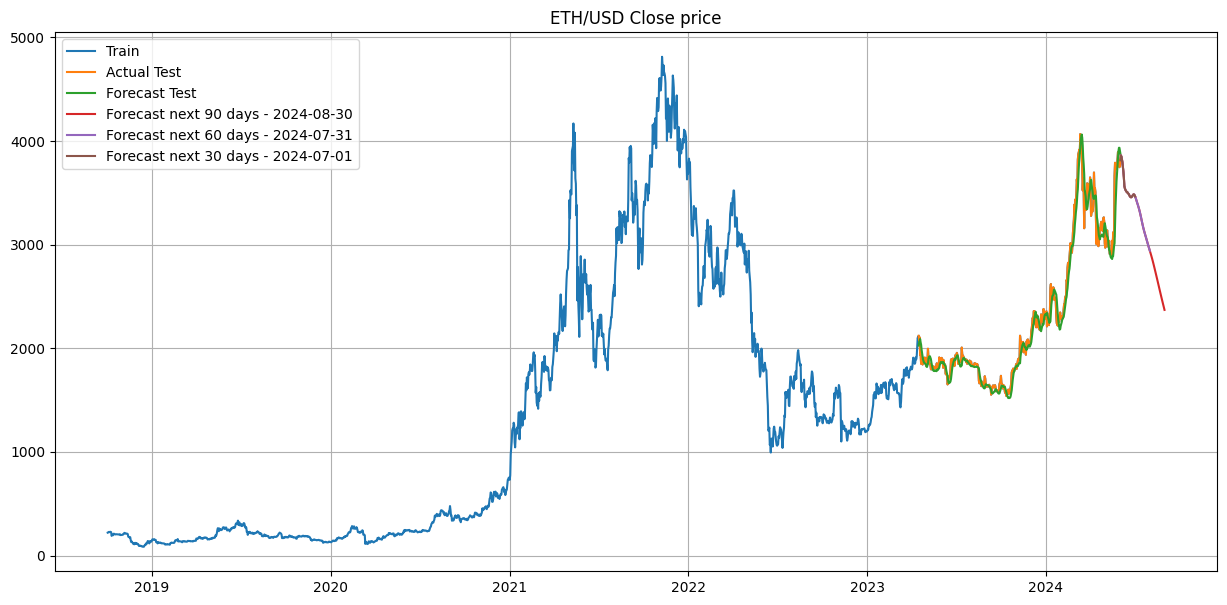
\includegraphics[width=0.8\linewidth]{./././visualize/LinearRegression/ETH-80-20.png} 
    \caption{Linear Regression model’s result with 8:2 ratio}
    \label{fig:21}
\end{figure}
\begin{figure}[H]
    \centering 
    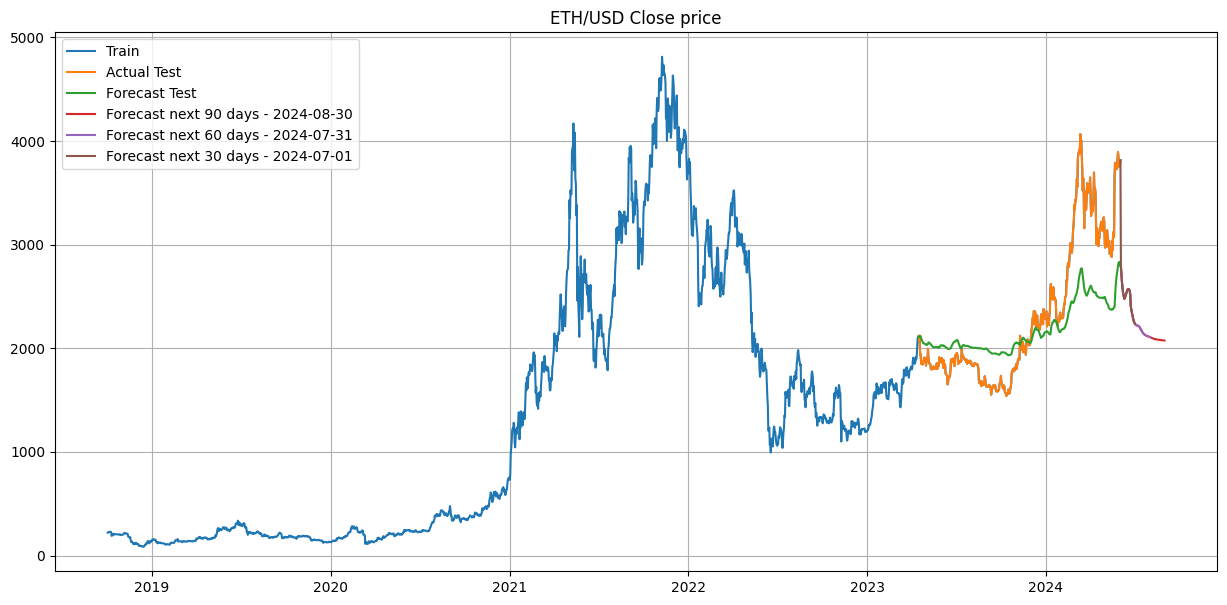
\includegraphics[width=0.8\linewidth]{./././visualize/ARIMAX/ETH-80-20.png} 
    \caption{ARIMAX model’s result with 8:2 ratio}
    \label{fig:22}
\end{figure}
\begin{figure}[H]
    \centering 
    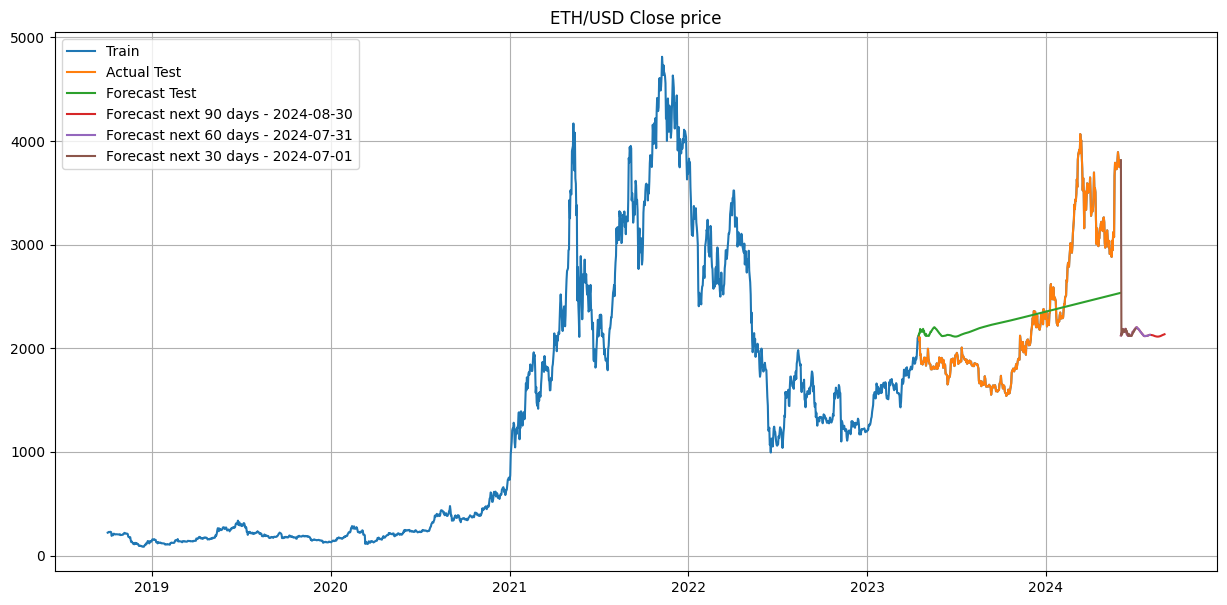
\includegraphics[width=0.8\linewidth]{./././visualize/VAR/ETH-80-20.png} 
    \caption{VAR model’s result with 8:2 ratio}
    \label{fig:23}
\end{figure}
%rnn 9:1
\begin{figure}[H]
    \centering 
    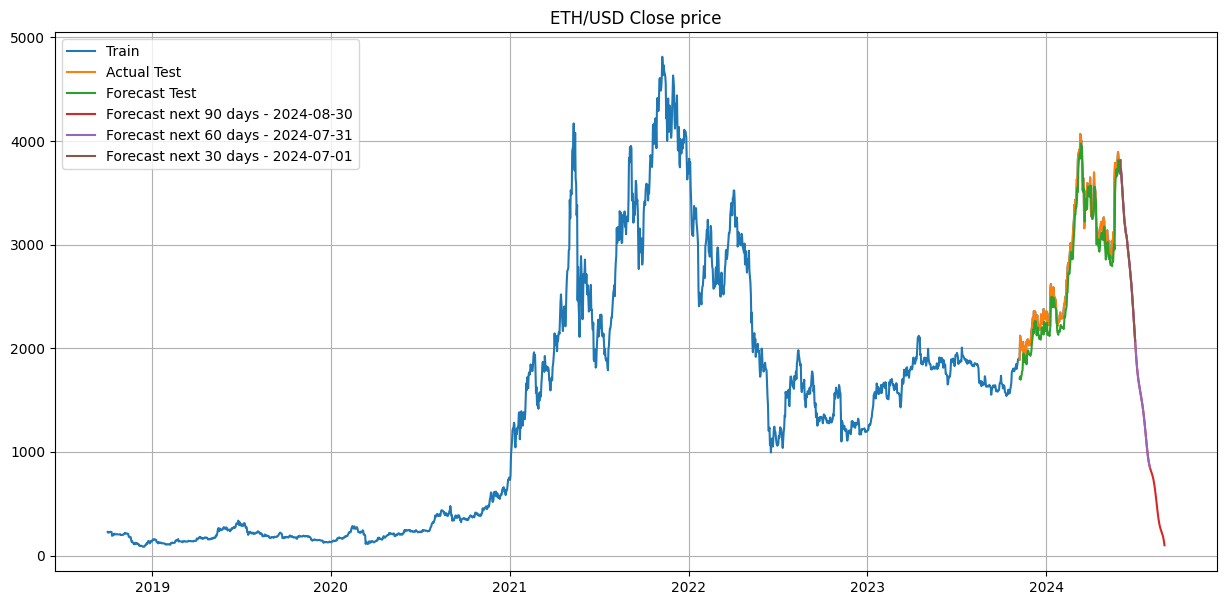
\includegraphics[width=0.8\linewidth]{./././visualize/RNN/ETH-90-10.png} 
    \caption{RNN model’s result with 9:1 ratio}
    \label{fig:24}
\end{figure}
%lstm 8:2
\begin{figure}[H]
    \centering 
    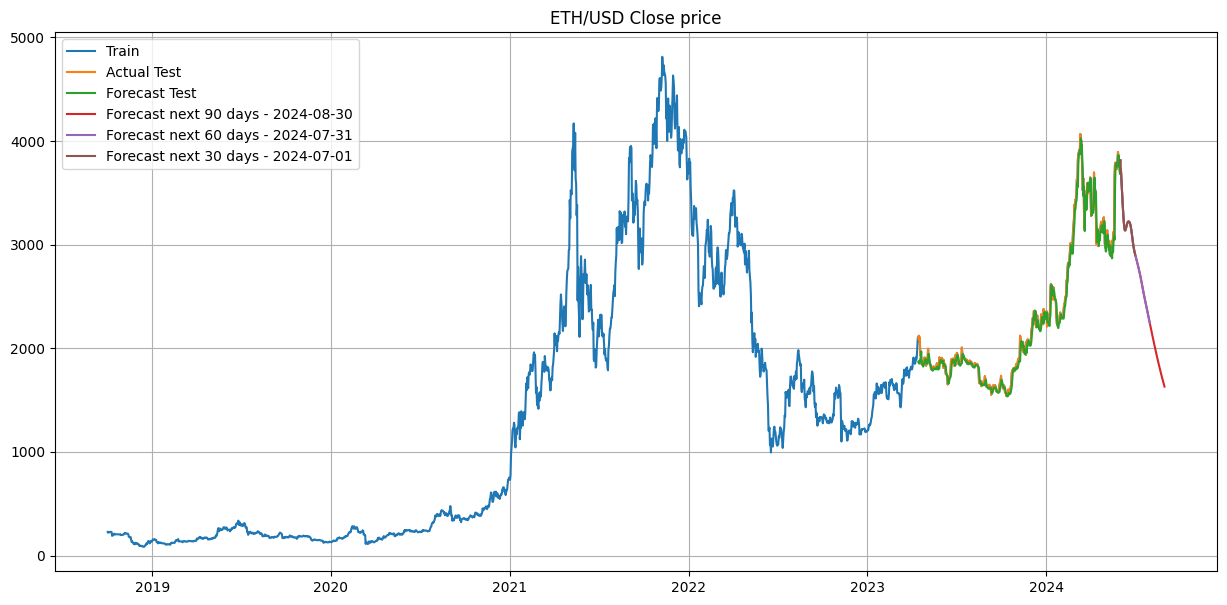
\includegraphics[width=0.8\linewidth]{./././visualize/LSTM/ETH-80-20.png} 
    \caption{LSTM model’s result with 8:2 ratio}
    \label{fig:25}
\end{figure}
%gru 8:2
\begin{figure}[H]
    \centering 
    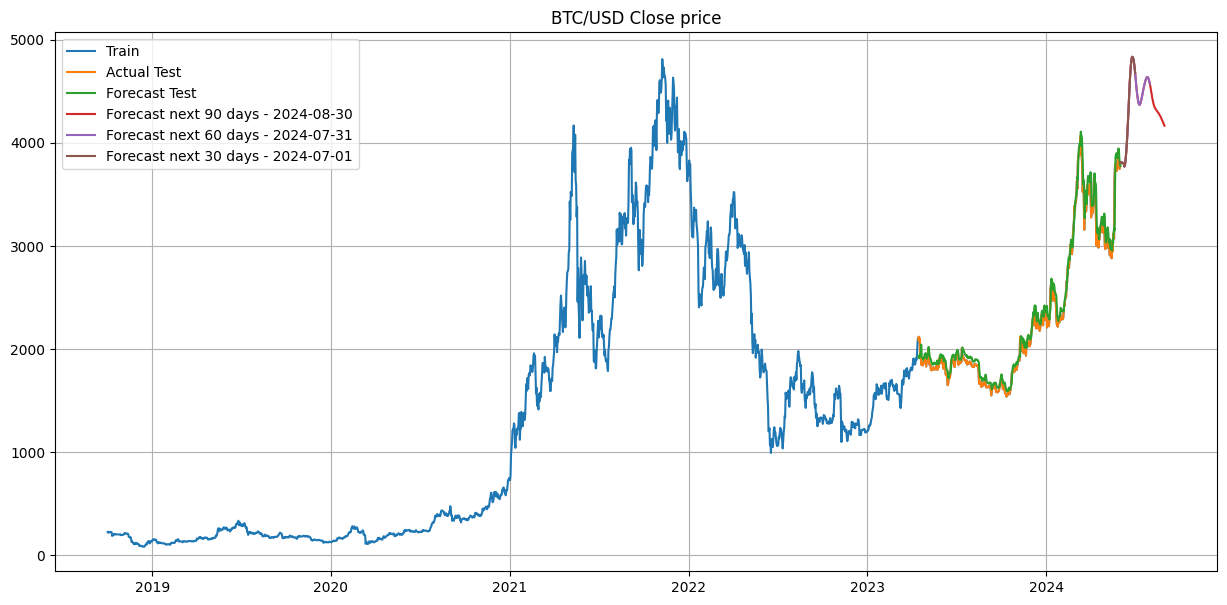
\includegraphics[width=0.8\linewidth]{./././visualize/GRU/ETH-80-20.png} 
    \caption{GRU model’s result with 8:2 ratio}
    \label{fig:26}
\end{figure}
%xgboost 8:2
\begin{figure}[H]
    \centering 
    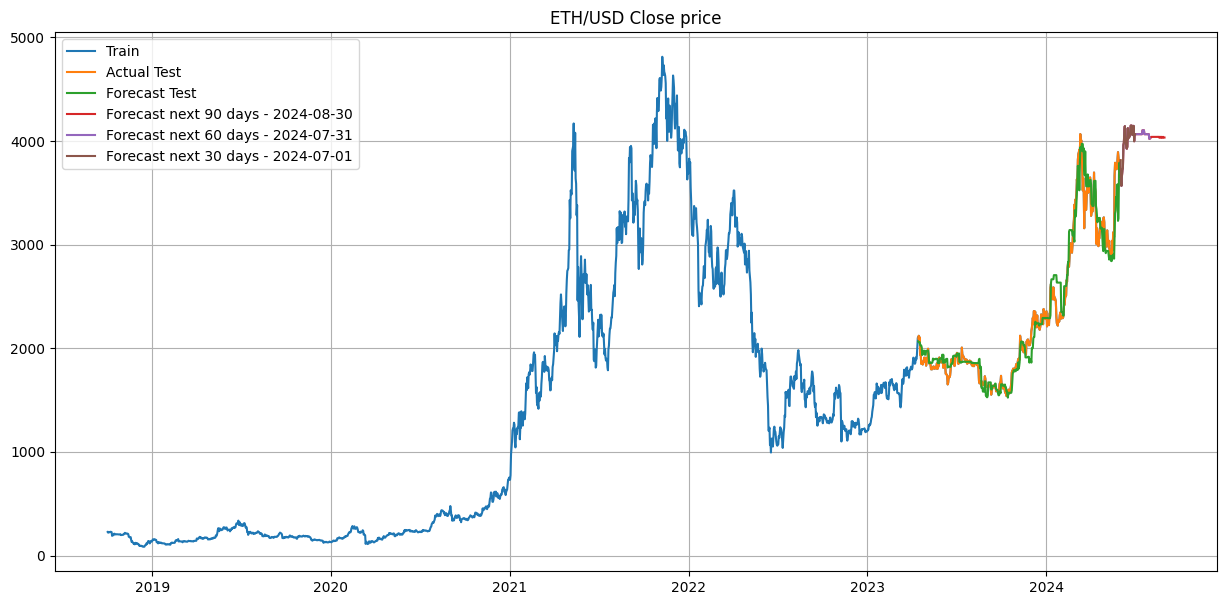
\includegraphics[width=0.8\linewidth]{./././visualize/XGBoost/ETH-80-20.png} 
    \caption{XGBoost model’s result with 8:2 ratio}
    \label{fig:27}
\end{figure}
%lightgbm 8:2
\begin{figure}[H]
    \centering 
    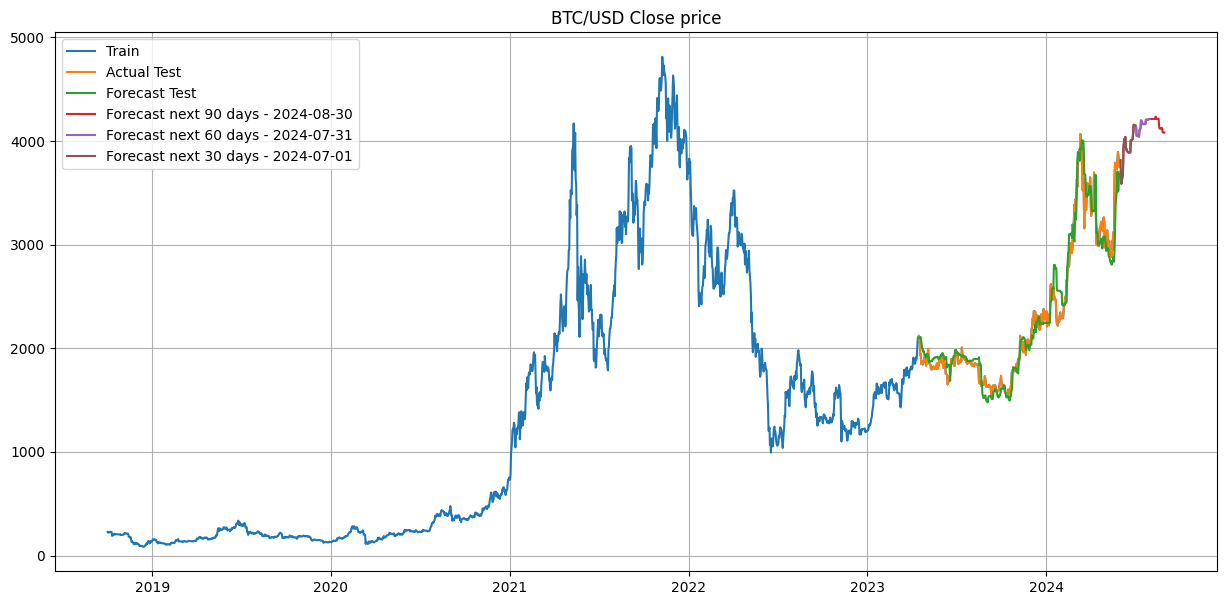
\includegraphics[width=0.8\linewidth]{./././visualize/LightGBM/ETH-80-20.png} 
    \caption{LightGBM model’s result with 8:2 ratio}
    \label{fig:28}
\end{figure}
\subsubsection{DOGE Dataset}
\begin{figure}[H]
    \centering 
    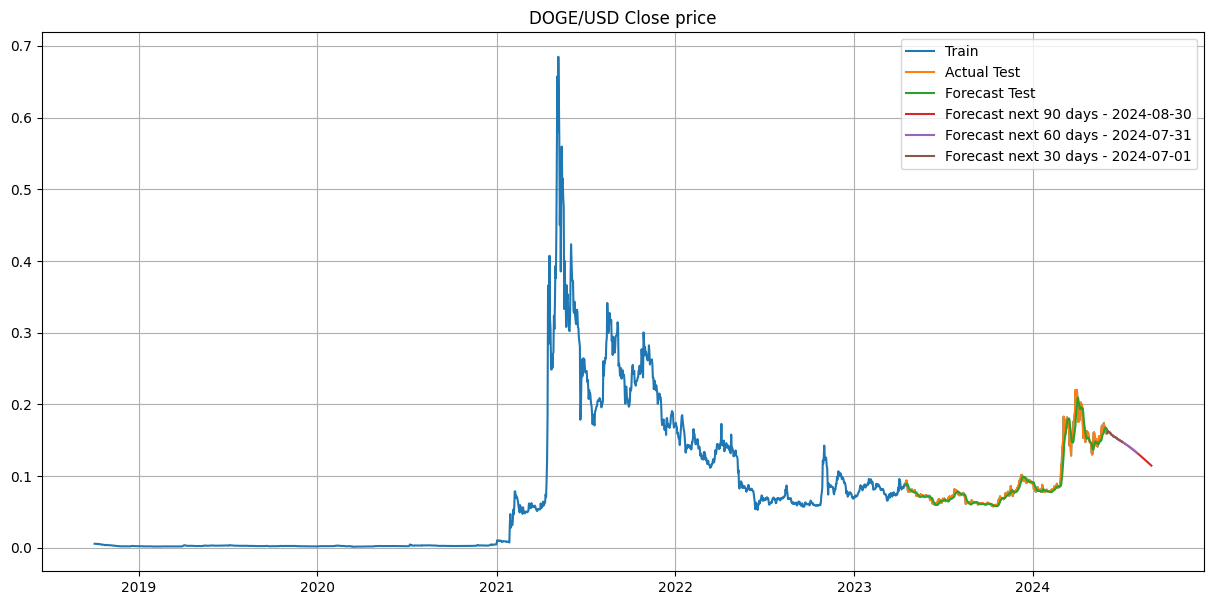
\includegraphics[width=0.8\linewidth]{./././visualize/LinearRegression/DOGE-80-20.png} 
    \caption{Linear Regression model’s result with 8:2 ratio}
    \label{fig:29}
\end{figure}
\begin{figure}[H]
    \centering 
    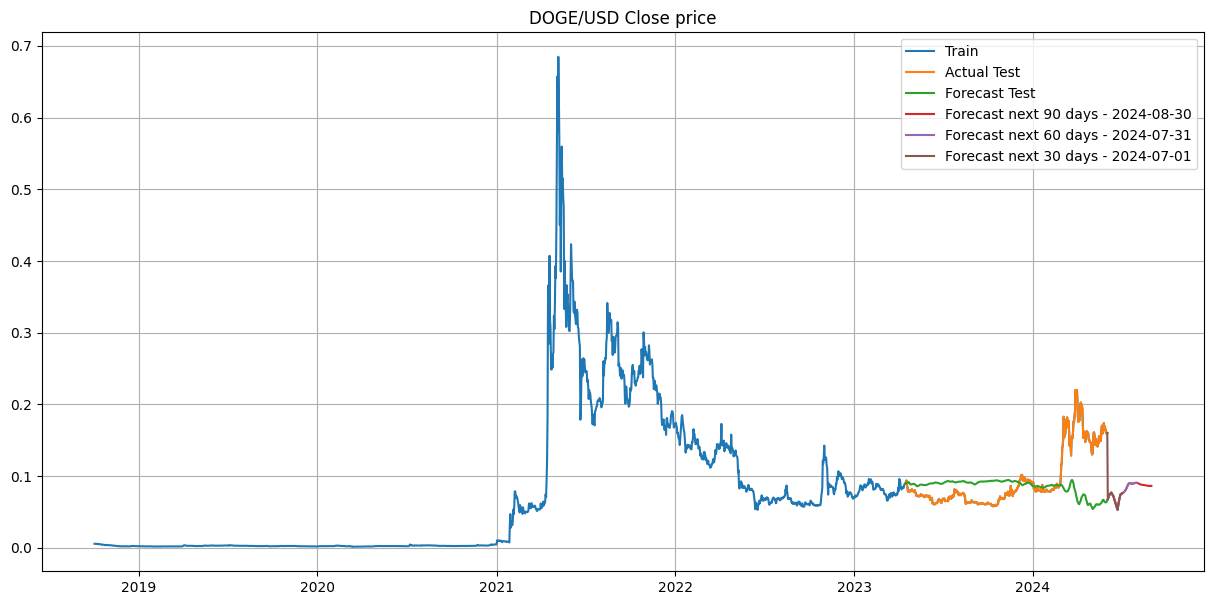
\includegraphics[width=0.8\linewidth]{./././visualize/ARIMAX/DOGE-80-20.png} 
    \caption{ARIMAX model’s result with 8:2 ratio}
    \label{fig:30}
\end{figure}
%var 7:3
\begin{figure}[H]
    \centering 
    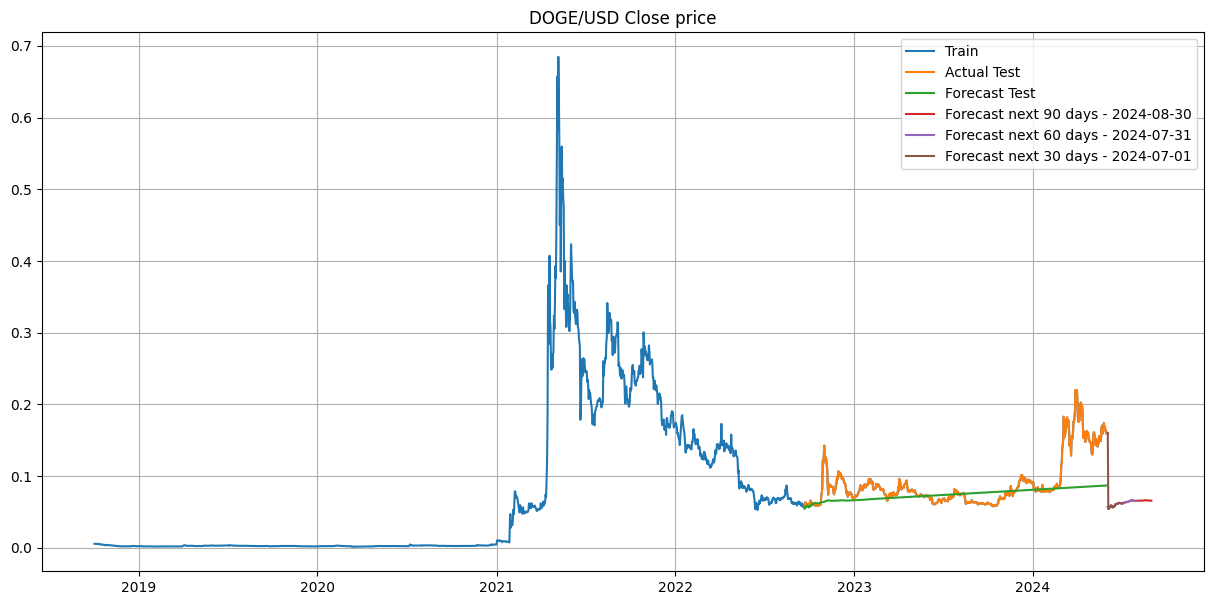
\includegraphics[width=0.8\linewidth]{./././visualize/VAR/DOGE-70-30.png} 
    \caption{VAR model’s result with 7:3 ratio}
    \label{fig:31}
\end{figure}
%rnn 9:1
\begin{figure}[H]
    \centering 
    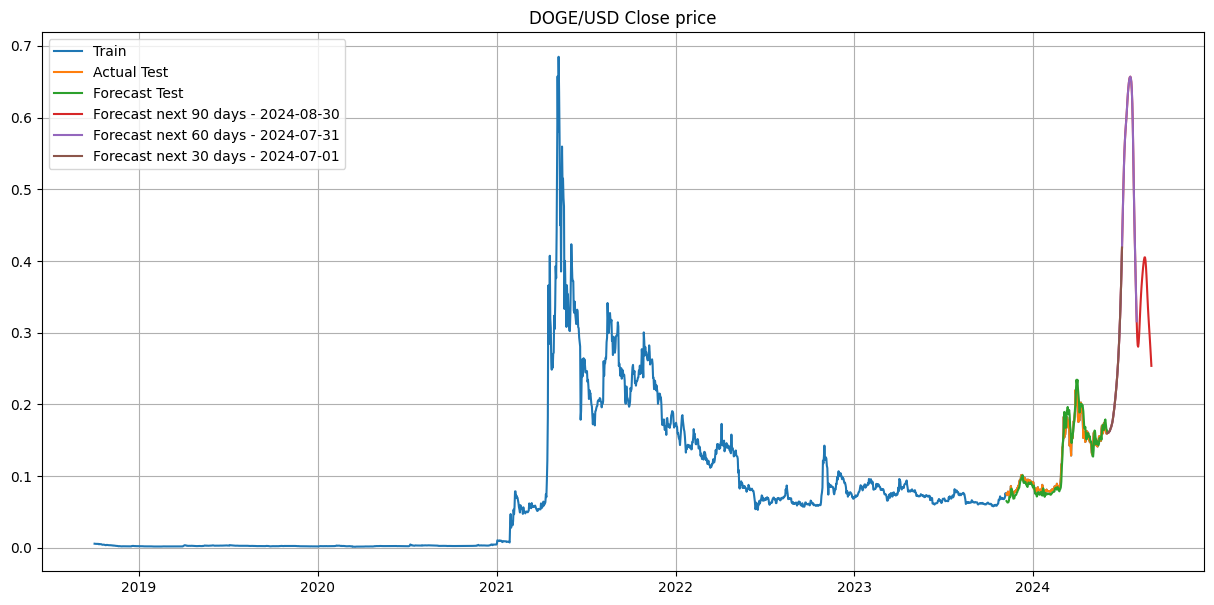
\includegraphics[width=0.8\linewidth]{./././visualize/RNN/DOGE-90-10.png} 
    \caption{RNN model’s result with 9:1 ratio}
    \label{fig:32}
\end{figure}
%lstm 9:1
\begin{figure}[H]
    \centering 
    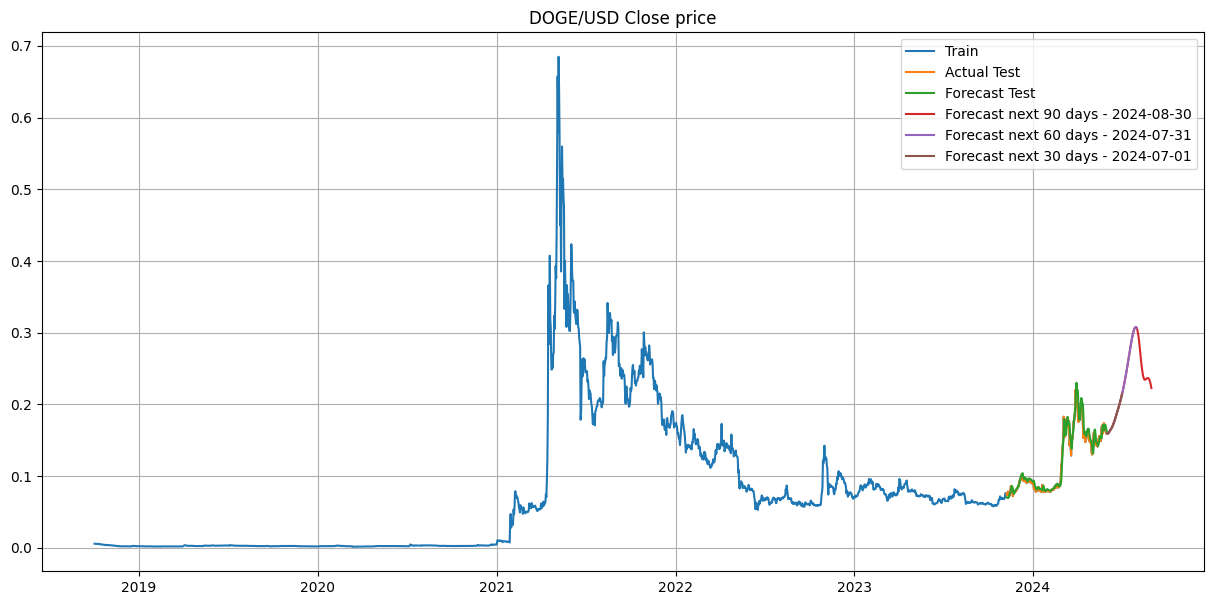
\includegraphics[width=0.8\linewidth]{./././visualize/LSTM/DOGE-90-10.png} 
    \caption{LSTM model’s result with 9:1 ratio}
    \label{fig:33}
\end{figure}
%gru 7:3
\begin{figure}[H]
    \centering 
    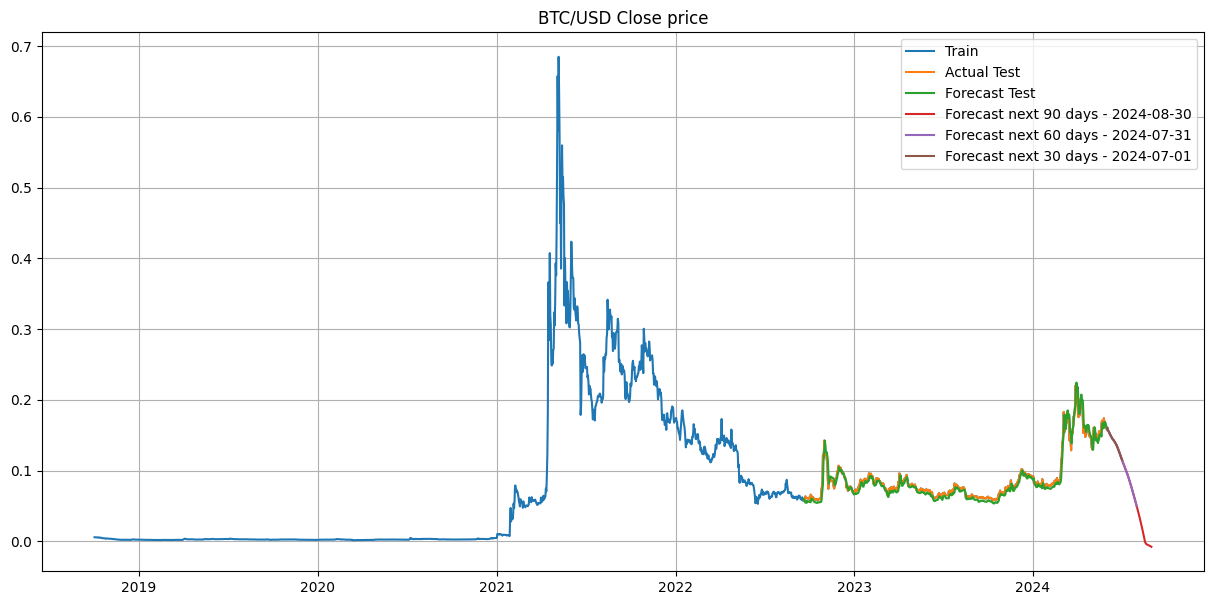
\includegraphics[width=0.8\linewidth]{./././visualize/GRU/DOGE-70-30.png} 
    \caption{GRU model’s result with 7:3 ratio}
    \label{fig:34}
\end{figure}
%xgboost 8:2
\begin{figure}[H]
    \centering 
    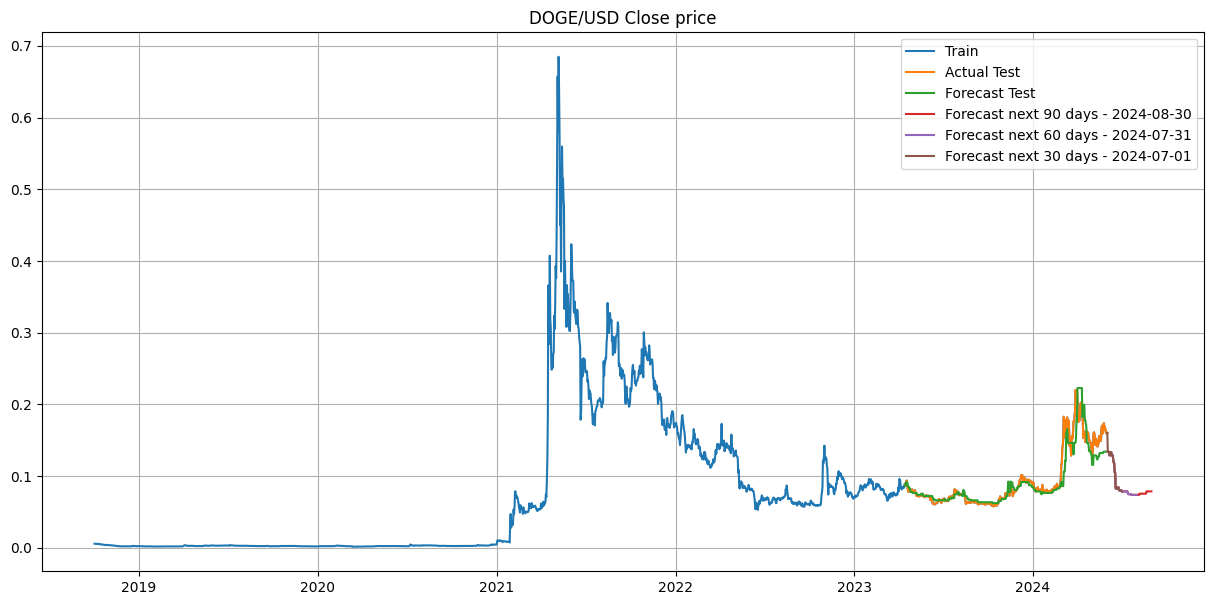
\includegraphics[width=0.8\linewidth]{./././visualize/XGBoost/DOGE-80-20.png} 
    \caption{XGBoost model’s result with 8:2 ratio}
    \label{fig:35}
\end{figure}
%lightgbm 8:2
\begin{figure}[H]
    \centering 
    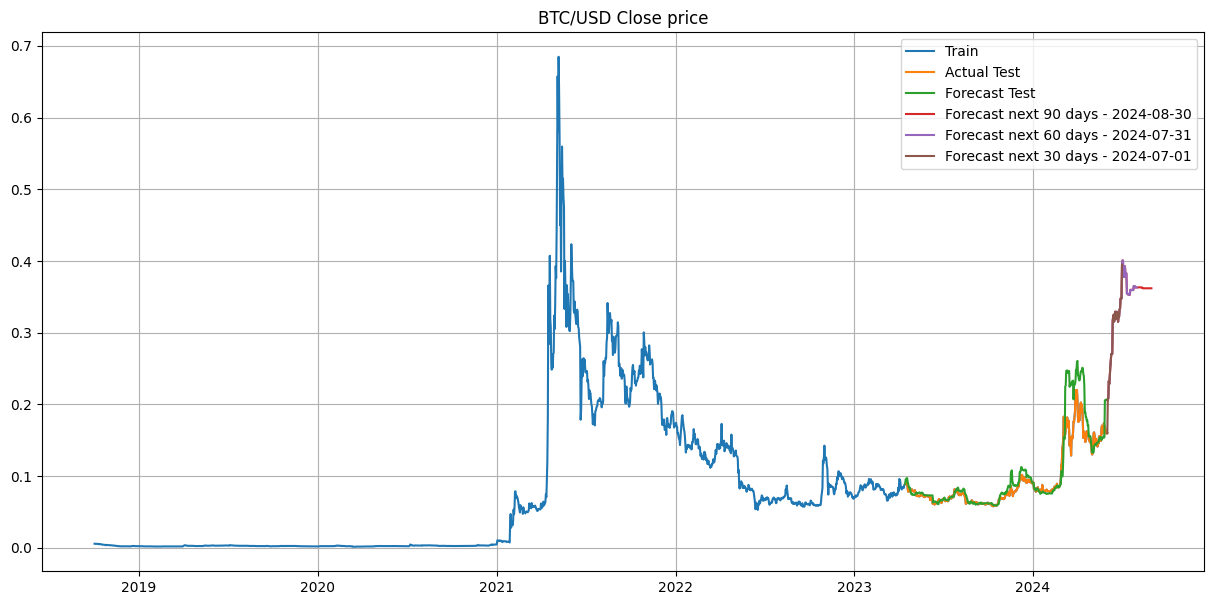
\includegraphics[width=0.8\linewidth]{./././visualize/LightGBM/DOGE-80-20.png} 
    \caption{LightGBM model’s result with 8:2 ratio}
    \label{fig:36}
\end{figure}
\section{Conclusion}
\subsection{Summary}
Machine learning models have emerged as a promising tool for accurately predicting and evaluating the value of cryptocurrencies, akin to their application in stock trading. In this study, we performed a detailed comparative analysis of various statistical and machine learning models to enhance cryptocurrency price prediction by integrating technical indicators. The models examined included Linear Regression, ARIMAX, RNN, GRU, LSTM networks, VAR, XGBoost, and LightGBM, using a dataset comprising Bitcoin (BTC), Ethereum (ETH), and Dogecoin (DOGE). Our evaluation metrics were RMSE, MAPE, and SMAPE, with GRU and LSTM models demonstrating exceptional performance in capturing the intricate patterns of cryptocurrency price movements.\\
However, the dataset used in this analysis is influenced by numerous factors such as market sentiment, regulatory news, macroeconomic trends, and technological advancements. These external factors can introduce noise and unpredictability, posing significant challenges for accurate price prediction. Consequently, as the best performing models among the eight models executed, GRU and LSTM may still face difficulties in maintaining consistent accuracy over time due to the inherent volatility and multifaceted nature of the cryptocurrency market.
\subsection{Future Consideration}
% Looking ahead, our team proposes the exploration of hybrid models that combine the strengths of various statistical and machine learning approaches. By continuously refining and exploring more models, we aim to develop more robust and reliable tools for forecasting cryptocurrency prices, thereby supporting traders and analysts in navigating this complex and dynamic market. In conclusion, machine learning models offer a promising approach to predict and evaluate the value of cryptocurrencies. Further research and advancements in this field can lead to more precise predictions and a deeper comprehension of the cryptocurrency market.
To advance our research in cryptocurrency price prediction, we aim to leverage a diverse range of technical indicators such as moving averages, oscillators, and volume-based metrics. By integrating these indicators, we seek to create a comprehensive dataset that captures the multifaceted dynamics of market behavior. This approach will facilitate the development of a sophisticated system capable of generating reliable buy/sell signals and forecasting future price trends, thereby assisting investors in minimizing risks effectively.
Our strategy includes exploring hybrid models that combine statistical methods with advanced machine learning algorithms like ARIMAX with GRU or LSTM networks. This integration aims to enhance forecast accuracy and robustness, ensuring our predictive system can adapt to the volatile nature of the cryptocurrency market. Continuous refinement through techniques such as hyperparameter tuning and ensemble learning will further strengthen the predictive performance, providing valuable tools for informed decision-making and risk management in cryptocurrency trading.




\section*{Acknowledgment}
We extend our heartfelt gratitude to Associate Professor Nguyen Dinh Thuan and T.A. Nguyen Minh Nhut for generously dedicating your time and expertise to guide us through the implementation of our project. Your invaluable suggestions and unwavering support were instrumental in our successful completion of the project. We are deeply thankful and privileged to have had the opportunity to learn under your guidance. Your significant contributions to our learning journey are sincerely appreciated. We look forward to continuing to receive your guidance and encouragement in the future.\\


%% UNCOMMENT these lines below (and remove the 2 commands above) if you want to embed the bibliografy.
\begin{thebibliography}{00}
    \bibitem{b1} Sun, G. (2024). Cryptocurrency price prediction based on Xgboost, LightGBM and BNN. \textit{Applied and Computational Engineering}, 49(1), 273–279. \url{https://doi.org/10.54254/2755-2721/49/20241414}

    \bibitem{b2} Yuan, Z. (2023). Gold and Bitcoin Price Prediction based on KNN, XGBoost and LightGBM Model. \textit{Highlights in Science, Engineering and Technology}, 39, 720–725. \url{https://doi.org/10.54097/hset.v39i.6635}

    \bibitem{b3} Haydier, E., Albarwari, N., \& Ali, T. H. (2023, December 1). The Comparison Between VAR and ARIMAX Time Series Models in Forecasting. \textit{Iraqi Journal of Statistical Sciences}. \url{https://doi.org/10.33899/iqjoss.2023.181260}

    \bibitem{b4} Dutta, A., Kumar, S. S., \& Basu, M. (2020). A gated Recurrent unit approach to bitcoin price prediction. \textit{Journal of Risk and Financial Management}, 13(2), 23. \url{https://doi.org/10.3390/jrfm13020023}

    \bibitem{b5} Gunarto, D. M., Saadah, S., \& Utama, D. Q. (2023). Predicting cryptocurrency price using RNN and LSTM method. \textit{Jurnal Sistem Informasi Dan Komputer/Jurnal Sisfokom}, 12(1), 1–8. \url{https://doi.org/10.32736/sisfokom.v12i1.1554}

    \bibitem{b6} Huang, J.-Z., Huang, W., \& Ni, J. (2019). Predicting bitcoin returns using high-dimensional technical indicators. \textit{The Journal of Finance and Data Science}, 5(3), 140–155. \url{https://doi.org/10.1016/j.jfds.2018.10.001}

    \bibitem{b7} Mudassir, M., Bennbaia, S., Ünal, D., \& Hammoudeh, M. (2020). Time-series forecasting of Bitcoin prices using high-dimensional features: a machine learning approach. \textit{Neural Computing and Applications}. \url{https://doi.org/10.1007/s00521-020-05129-6}

    \bibitem{b8} Liao, S. (2023). Predicting the price of Bitcoin, Dogecoin and Ethereum by machine learning. \textit{BCP Business \& Management, 38, 3389–3395}. \url{https://doi.org/10.54691/bcpbm.v38i.4312}

    \bibitem{b9} Guo, X., Ha, M., Tao, X., Li, S., Li, Y., Zhu, Z., Shen, Z., \& Ma, L. (2024). Multi-Task Learning with Sequential Dependence Toward Industrial Applications: A Systematic Formulation. \textit{ACM Transactions on Knowledge Discovery from Data, 18(5), 1-29}. \url{https://doi.org/10.1145/3640468}
    \bibitem {b10} Demir, S., Mincev, K., Kok, J., \& Paterakis, N. G. (2019). Introducing Technical Indicators to Electricity Price Forecasting: A feature engineering study for linear, ensemble, and deep machine learning models. \textit{Applied Sciences, 10(1), 255}. \url{https://doi.org/10.3390/app10010255}

    \bibitem{b11} Chen, T., \& Guestrin, C. (2016, August). Xgboost: A scalable tree boosting system. \textit{In Proceedings of the 22nd acm sigkdd international conference on knowledge discovery and data mining (pp. 785-794).} 
    
    \bibitem{12} Agrawal, M., Shukla, P. K., Nair, R., Nayyar, A., \& Masud, M. (2022). Stock prediction based on technical indicators using deep learning model. \textit{Computers, Materials \& Continua/Computers, Materials \& Continua (Print), 70(1), 287–304}. \url{https://doi.org/10.32604/cmc.2022.014637} 

    \bibitem{13} Vol. 12 No. 3 (2024) | \textit{International Journal of Intelligent Systems and Applications in Engineering. (2023c, March 6)}. \url{https://ijisae.org/index.php/IJISAE/issue/view/126}

    \bibitem{14} Bagade, K., \& Bhosale, V. (2022). Artificial Intelligence based Stock Market Prediction Model using Technical Indicators. \textit{International Journal of Innovative Technology and Exploring Engineering, 11(6), 34–39}. \url{https://doi.org/10.35940/ijitee.f9915.0511622}

    \bibitem{15} Htun, H. H., Biehl, M., \& Petkov, N. (2023). Survey of feature selection and extraction techniques for stock market prediction. \textit{Financial Innovation, 9(1)}. \url{https://doi.org/10.1186/s40854-022-00441-7}

    

\end{thebibliography}

\EOD

\end{document}
